\documentclass[9pt,a4paper,twocolumn]{article}
% The following LaTeX packages must be installed on your machine: amsmath, authblk, bm, booktabs, caption, dcolumn, fancyhdr, geometry, graphicx, hyperref, latexsym, natbib
\input{151.dat}
\usepackage{gensymb}
\usepackage{amsthm}
\usepackage{float}
\usepackage{siunitx}
\usepackage{amssymb}
\usepackage{float}
\usepackage{enumerate}
\usepackage{listings}
\usepackage{mathtools}
\PassOptionsToPackage{hyphens}{url}\usepackage{hyperref}
\usepackage[none]{hyphenat}
\usepackage{physics}
\usepackage{chngcntr}
\counterwithin*{equation}{section}
\counterwithin*{equation}{subsection}
\newcommand\ddfrac[2]{\frac{\displaystyle #1}{\displaystyle #2}}
%\renewcommand{\familydefault}{\sfdefault}


\begin{document}

\begin{titlepage}
\begin{center}
\vspace*{\fill}

\normalsize{Physics 151 \\
Crib Sheet \\
2nd semester, A.Y. 2018-19} \\

\qquad
\qquad

\normalsize{Kenneth V. Domingo \\
2015-03116 \\
28}

\vspace*{\fill}
\end{center}
\end{titlepage}

\tableofcontents

\clearpage

\setcounter{page}{1}

\section{P09 PS02 2.8 Work in a cyclic process}
Consider the cyclic process as described in Example 2.1.

\begin{figure}[htb]
	\centering
	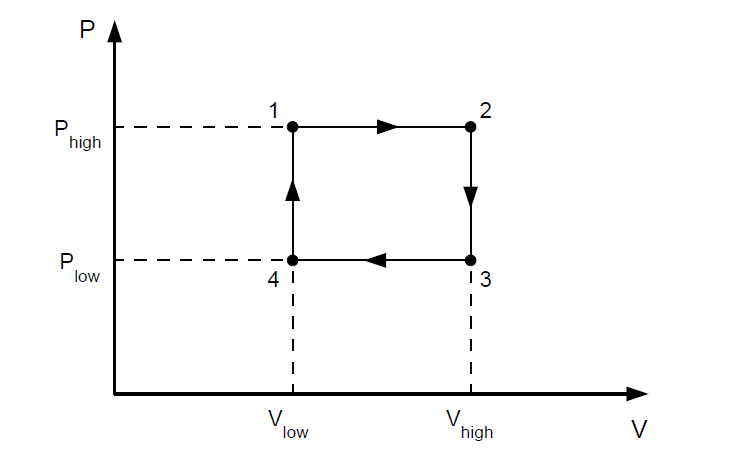
\includegraphics[width=0.75\linewidth]{work.png}
	\caption{Cyclic process for this problem.}
	\label{fig:2.8-cycle}
\end{figure}

\begin{enumerate}[(a)]
	\item Because the system was returned to its original pressure and volume, why is the net amount of work done on the system not zero?
	
	The net work done on the system is non-zero since it depends on the initial, intermediate, and final macrostates (i.e. the path).
	
	\item What would be the work done on the gas if the gas were taken from $1 \rightarrow 2 \rightarrow 3$ and then back to 1 along the diagonal path connecting 3 and 1?

\begin{align}
	W_{1 \rightarrow 2} &= P_{high}\qty(V_{high} - V_{low}) \\
	W_{2 \rightarrow 3} &= \qty(P_{low} - P_{high})V_{high} \\
	W_{3 \rightarrow 1} &= \sqrt{P_{high}^2\qty(V_{high} - V_{low})^2 + \qty(P_{low} - P_{high})^2 V_{high}^2} \\
	W_{net} &= W_{1 \rightarrow 2} + W_{2 \rightarrow 3} + W_{3 \rightarrow 1}
\end{align}

\end{enumerate}


\section{P10 PS02 2.13}
In Example 2.1 we showed that the net work done on the gas in the cyclic process shown in Figure \ref{fig:2.8-cycle} is nonzero. Assume that the gas is ideal with N particles and calculate the energy transfer by heating in each step of the process. Then explain why the net work done on the gas is negative and show that the net change of the internal energy is zero.

From Example 2.1, the net work done on a gas in a cyclic process was determined to be nonzero, with a value of

\begin{equation}\label{oldanswer}
	W_{net} = -\left( P_{high} - P_{low} \right) \left( V_{high} - V_{low} \right)
\end{equation}

Assuming an ideal gas with $N$ particles, the energy transfer due to heating for each step in the process is as follows:

\begin{align}
	Q_{1 \rightarrow 2} = -Q_{3 \rightarrow 4} & = \int_{T_1}^{T_2} c_P \textrm{ d}T \\
	& = \nu c_P \int_{T_1}^{T_2} \textrm{ d}T \\
	& = \nu c_P \left( T_2 - T_1 \right) \\
	& = \nu c_P \Delta T \label{eq:isobaric} \\
	Q_{2 \rightarrow 3} = -Q_{4 \rightarrow 1} & = \int_{T_1}^{T_2} c_V \textrm{ d}T \\
	& = \nu c_V \int_{T_1}^{T_2} \textrm{ d}T \\
	& = \nu c_V \left( T_2 - T_1 \right) \\
	& = \nu c_V \Delta T \label{eq:isochoric}
\end{align}

Recalling the ideal gas equation,

\begin{eqnarray}
	PV = \nu RT \label{eq:idealgas} \\
	T = \frac{PV}{\nu R} \label{eq:idealtemp}
\end{eqnarray}

The net energy transfer due to heating is

\begin{equation}\label{eq:totalwork}
	W_{net} = Q_{1 \rightarrow 2} + Q_{2 \rightarrow 3} + Q_{3 \rightarrow 4} + Q_{4 \rightarrow 1}
\end{equation}

Plugging \eqref{eq:idealtemp} into each of the equations in \eqref{eq:isobaric} and \eqref{eq:isochoric}, we have

\begin{align}
	Q_{1 \rightarrow 2} & = \nu c_P P_{high} \frac{V_{high} - V_{low}}{\nu R} \label{eq:Q12plug} \\
	Q_{2 \rightarrow 3} & = \nu c_V V_{high} \frac{P_{low} - P_{high}}{\nu R} \label{eq:Q23plug} \\
	Q_{3 \rightarrow 4} & = \nu c_P P_{low} \frac{V_{low} - V_{high}}{\nu R} \label{eq:Q34plug} \\
	Q_{4 \rightarrow 1} & = \nu c_V V_{low} \frac{P_{high} - P_{low}}{\nu R} \label{eq:Q41plug}
\end{align}

Simplifying equations \eqref{eq:Q12plug} through \eqref{eq:Q41plug} and summing them as in \eqref{eq:totalwork}, we have

\begin{align}
	Q_{net} & = c_P P_{high} \frac{V_{high} - V_{low}}{R} \nonumber \\
	& - c_V V_{high} \frac{P_{high} - P_{low}}{R} \nonumber \\
	& - c_P P_{low} \frac{V_{high} - V_{low}}{R} \nonumber \\
	& + c_V V_{low} \frac{P_{high} - P_{low}}{R}
\end{align}
\begin{align}
	Q_{net} & = \frac{c_P}{R} \left( P_{high} - P_{low} \right) \left( V_{high} - V_{low} \right) \nonumber \\
	& -\frac{c_V}{R} \left( P_{high} - P_{low} \right) \left( V_{high} - V_{low} \right) \label{eq:Wnetplug}
\end{align}

Recall that for an ideal gas,

\begin{eqnarray}
	c_P = \frac{5}{2} R \label{eq:idealcp} \\
	c_V = \frac{3}{2} R \label{eq:idealcv}
\end{eqnarray}

Plugging these into \eqref{eq:Wnetplug},

\begin{align}
	Q_{net} & = \frac{5}{2} R \frac{1}{R} \left( P_{high} - P_{low} \right) \left( V_{high} - V_{low} \right) \nonumber \\
	& -\frac{3}{2} R \frac{1}{R} \left( P_{high} - P_{low} \right) \left( V_{high} - V_{low} \right) \label{eq:Wnetideal}
\end{align}

Which gives us the expected relation of $Q_{net} = -W_{net}$ (negative because in a cyclic process, there is no change in internal energy; the work done is equal to the heat added):

\begin{equation}\label{eq:answer}
	Q_{net} = \left( P_{high} - P_{low} \right) \left( V_{high} - V_{low} \right)
\end{equation}

From the first thermodynamic law,

\begin{equation}\label{eq:1stlaw}
	\Delta E = Q + W
\end{equation}

Plugging equations \eqref{oldanswer} and \eqref{eq:answer} into this, we have

\begin{equation}\label{eq:energychange}
	\Delta E = 0
\end{equation}

\section{P11 PS03 2.15}
Use (2.44) and the ideal gas pressure equation of state in (2.8) to show that in a quasistatic adiabatic processes $P$ and $V$ are related as

\begin{equation}
	PV^\gamma = \textrm{constant}
\end{equation}

Also show that $T$ and $P$ are related as

\begin{equation}
	TP^{(1-\gamma)/\gamma} = \textrm{constant}
\end{equation}

The given equations are:

\begin{eqnarray}
	TV^{\gamma-1} = C \label{eq:given1} \\
	PV = \nu RT \label{eq:idealgaslaw}
\end{eqnarray}

Isolating $T$ in \eqref{eq:idealgaslaw},

\begin{equation}
	T = \frac{PV}{\nu R} \label{eq:idealgastemp}
\end{equation}

Plugging this into \eqref{eq:given1},

\begin{align}
	\frac{PV}{\nu R} V^{\gamma - 1} = C \nonumber \\
	PV^{\gamma} = C\nu R = C
\end{align}

Therefore,

\begin{equation}\label{eq:answer1}
\boxed{	PV^\gamma = \textrm{constant}}
\end{equation}

Similarly, isolating $V$ from \eqref{eq:idealgaslaw},

\begin{equation}\label{eq:idealgasvol}
	V = \frac{\nu RT}{P}
\end{equation}

Plugging this into \eqref{eq:answer1},

\begin{align}
	P\left( \frac{\nu RT}{P} \right)^\gamma & = C \nonumber \\
	\left( \nu RT \right)^\gamma P^{1-\gamma} & = C \nonumber \\
	T^\gamma P^{1-\gamma} & = \frac{C}{\left( \nu R \right)^\gamma} \nonumber \\
	T^\gamma P^{1-\gamma} & = D
\end{align}

Raising both sides to $1/\gamma$,

\begin{eqnarray}
	\left( T^\gamma P^{1-\gamma} \right)^{\frac{1}{\gamma}} = D^{\frac{1}{\gamma}} \nonumber \\
\boxed{	TP^{(1 - \gamma)/\gamma} = \textrm{constant}} \label{eq:answer2}
\end{eqnarray}

\section{P12 PS03 2.17 Compression of air}
\begin{enumerate}[(a)]

\item Air initially at $20^\circ$C is compressed by a factor of 15. Assuming adiabatic conditions, $V_i/15 = V_f$, $T_i = 293$K, and $\gamma = 1.4$,

\begin{eqnarray}
	TV^{\gamma -1} = C \label{eq:adiabatic} \\
	T_i V_i^{\gamma-1} = T_f V_f^{\gamma - 1} \nonumber \\
	293 V_i^{0.4} = T_f \left( \frac{V_i}{15} \right)^{0.4} \nonumber \\
	293 = T_f \left(\frac{1}{15}\right)^{0.4} \nonumber \\
	T_f = 293 \left( \frac{1}{15} \right)^{-0.4} \nonumber \\
	\boxed{T_f = 866\textrm{ K}} \label{eq:answer1}
\end{eqnarray}

Assuming air behaves like an ideal gas,

\begin{eqnarray}
	\frac{P_i V_i}{T_i} = \frac{P_f V_f}{T_f} \\
	\frac{P_i}{293}\frac{V_f}{15} = \frac{P_f V_f}{866} \nonumber \\
	\frac{P_i}{(293)(15)} = \frac{P_f}{866} \nonumber \\
	\boxed{P_i \approx 5 P_f} \label{eq:answer2}
\end{eqnarray}

	\item If the compression is isothermal,

\begin{eqnarray}
	P_i V_i = P_f V_f \\
	\boxed{P_i = 15 P_f} \label{eq:answer3}
\end{eqnarray}

	\item The pressure increases more with adiabatic compression.

\end{enumerate}

\section{P13 PS03 2.18 Work done in a quasistatic adiabatic process}

\begin{enumerate}[(a)]

\item Use the result that we derived in (2.53) to obtain the alternative form (2.54).

From the given equations,

\begin{eqnarray}
	W = C_V \left( T_2 - T_1 \right) \label{eq:workvol} \\
	PV = \nu RT \label{eq:idealgas} \\
	C_V = \frac{3}{2} \nu k_B \label{eq:volenergy}
\end{eqnarray}

Plugin \eqref{eq:idealgas} and \eqref{eq:volenergy} into \eqref{eq:workvol}:

\begin{align}
	W & = \frac{3}{2} \nu k_B \left( \frac{P_2 V_2}{\nu k_B} - \frac{P_1 V_1}{\nu k_B} \right) \nonumber \\
	& = \frac{3}{2} \left( P_2 V_2 - P_1 V_1 \right)
\end{align}

Since $\gamma = \frac{5}{3}$ for monatomic ideal gas,

\begin{align}
	W & = \frac{\left( P_2 V_2 - P_1 V_1 \right)}{\frac{2}{3}} \nonumber \\
	& = \frac{\left( P_2 V_2 - P_1 V_1 \right)}{\frac{5}{3} - \frac{3}{3}} \nonumber \\
	\Aboxed{ W & = \frac{\left( P_2 V_2 - P_1 V_1 \right)}{\gamma - 1}} \label{eq:answer1}
\end{align}

\item Show that another way to derive (2.54) is to use the relations (2.14) and (2.46).

From the given equations,

\begin{eqnarray}
	PV^\gamma = C \label{eq:constant} \\
	W = -\int_{V_1}^{V_2} P(T,V) \dd{V} \label{eq:workint}
\end{eqnarray}

Isolate $P$ from \eqref{eq:constant} and plug into \eqref{eq:workint}:

\begin{align}
	W &= -\int_{V_1}^{V_2} C V^{-\gamma} \dd{V} \nonumber \\
	& = -C \frac{V^{1 - \gamma}}{1 - \gamma} \bigg|_{V_1}^{V_2} \nonumber \\
	& = \frac{1}{\gamma - 1}\left( CV_2^{1-\gamma} - CV_1^{1-\gamma} \right) \nonumber \\
	& = \frac{1}{\gamma - 1}\left( CV_2^{-\gamma}V_2 - CV_1^{-\gamma}V_1 \right)
\end{align}

From \eqref{eq:constant},

\begin{equation}
	P = CV^{-\gamma}
\end{equation}

Therefore,

\begin{equation}\label{eq:answer2}
\boxed{	W = \frac{1}{\gamma - 1} \left( P_2 V_2 - P_1 V_1 \right) }
\end{equation}

\end{enumerate}

\section{P14 PS03 2.20 Heat pump}
A heat pump works on the same principle as a refrigerator, but the goal is to heat a room by cooling its cooler surroundings. For example, we could heat a building by cooling a nearby body of water. If we extract energy $Q_{cold}$ from the surroundings at $T_{cold}$, do work $W$, and deliver $Q_{hot}$ to the room at $T_{hot}$, the coefficient of performance is given by

\begin{equation}
	\textrm{COP} = \frac{\textrm{what you get}}{\textrm{what you pay for}} = \frac{Q_{hot}}{W}
\end{equation}

What is the maximum value of COP for a heat pump in terms of $T_{cold}$ and $T_{hot}$? What is the COP when the outside temperature is 0$^\circ$C and the interior temperature is 23$^\circ$C? Is it more effective to operate a heat pump during the winters in New England where the winters are cold or in the Pacific Northwest where the winters are relatively mild? (It is too bad that the maximum efficiency of a heat pump occurs when it is needed least.)

Since we want to heat a room surrounded by a cooler environment, the work done is positive:

\begin{align}
	\textrm{COP} &= \frac{Q_{hot}}{Q_{hot} - Q_{cold}} \\
	&= \frac{N k_B T_{hot} \ln{\left( \frac{V_f}{V_i} \right)}}{Nk_B T_{hot}\ln{\left( \frac{V_f}{V_i} \right)} - Nk_B T_{cold} \ln{\left( \frac{V_f}{V_i} \right)}} \nonumber  \\
	\Aboxed{\textrm{COP} &= \frac{T_{hot}}{T_{hot} - T_{cold}}} \label{eq:answer1}
\end{align}

Plugging the given conditions $T_{hot} = 296$K and $T_{cold} = 273$K into \eqref{eq:answer1},

\begin{align}
	\textrm{COP} &= \frac{296}{296-273} \nonumber \\
	\Aboxed{\textrm{COP} &= 12.9} \label{eq:answer2}
\end{align}

The denominator is larger for large temperature differences. The heater is more efficient in regions with mild winters.

\section{P15 PS03 2.21 Water in contact with two heat baths in succession}
The temperature of 1 kg of water at 0$^\circ$C is increased to 50$^\circ$C by first bringing it into contact
with a heat bath at 25$^\circ$C and then with a heat bath at 50$^\circ$C. What is the change in entropy of the entire system? How does this change in entropy compare with the change that was found in Example 2.15?

For the first bath,

\begin{align}\label{eq:entropy1}
	\Delta S_{11} &= C\ln{\left( \frac{T_b}{T_a} \right)} \\
	&= 4184\ln{\left( \frac{298}{273} \right)} \nonumber \\
	&= 366.6 \textrm{ J/K}
\end{align}

The energy transfer is

\begin{align}
	Q &= C \left( T_b - T_a \right) \\
	&= 4184(25) \nonumber \\
	&= 104,600 \textrm{ J}
\end{align}

So the entropy of the first bath is

\begin{align}
	\Delta S_{12} &= -\frac{Q}{T_b} \\
	&= -\frac{104 600}{298} \nonumber \\
	&= -351 \textrm{ J/K}
\end{align}

The total entropy change for the first bath is

\begin{align}
	\Delta S_1 &= 366.6 - 351 \\
	&= 15.6 \textrm{ J/K}
\end{align}

Similarly, for the second bath,

\begin{align}
	\Delta S_{21} &= 4184\ln{\left( \frac{323}{298} \right)} \\
	&= 337.1 \textrm{ J/K} \\
	\Delta S_{22} &= -\frac{Q}{T_b} \\
	&= -\frac{104 600}{323} \\
	&= -323.8 \textrm{ J/K} \\
	\Delta S_2 &= 337.1 - 323.8 \\
	&= 13.3 \textrm{ J/K}
\end{align}

The total entropy change for both processes is then

\begin{align}
	\Delta S &= 15.6 + 13.3 \\
\Aboxed{\Delta S&= 28.9 \textrm{ J/K}} \label{eq:answer1}
\end{align}


The value obtained is less than that of the water directly placed in contact with the $50^\circ$ bath.

\section{P16 PS04 2.23 More work}
\begin{enumerate}[(a)]

\item Show that the work performed by the heat engine in Example 2.19 is given by

\begin{equation}
	W = C_A \left( T_A - T \right) + C_B \left( T_B - T \right) \label{eq:prove}
\end{equation}

where $C_A$ and $C_B$ are constants and $T$ is given by (2.109) if the process is reversible. (Recall that our convention is to consider the work done on a system, except when we are discussing heat engines.)

Given

\begin{equation}\label{eq:giventemp}
	T = T_A^{\frac{C_A}{C_A + C_B}} T_B^{\frac{C_B}{C_A + C_B}}
\end{equation}

The work done by an engine on bath A for the entire process is

\begin{equation}\label{eq:workengine}
	W = -P\dd{V}
\end{equation}

From the ideal gas law,

\begin{align}
	PV = NkT \\
	\dd(PV) = \dd(NkT) \\
	P\dd{V} = Nk \dd{T} \label{eq:idealgas}
\end{align}

the temperature of bath A, from $T_A$, approaches the equilibrium temperature $T$. Express $\dd{V}$ as

\begin{equation}
	\dd{V} = \frac{Nk_B \dd{T}}{P}
\end{equation}

Plugging this into \eqref{eq:workengine},

\begin{align}
	W & = -P \frac{Nk_B\dd{T}}{P} \nonumber \\
	& = -Nk_B\dd{T} \nonumber \\
	& = -Nk_B \left( T - T_A \right) \nonumber \\
	& = Nk_B \left( T_A - T \right)
\end{align}

Define $C_A = N_A k_B$ as a constant inherent to bath A. The work done on bath A is

\begin{equation}
	W_A = C_A \left( T_A - T \right)
\end{equation}

Since the engine also does work on bath B, we can similarly define a constant inherent to bath B as $C_B = N_B k_B$. Consequently, 

\begin{equation}
	W_B = C_B \left( T_B - T \right)
\end{equation}

Thus, the total work done by the engine is

\begin{eqnarray}
	W = W_A + W_B \\
	\Aboxed{ W = C_A \left( T_A - T \right) + C_B \left( T_B - T \right) } \label{eq:answer-a}
\end{eqnarray}

\item Suppose that $C_A = C_B = C$ (a constant independent of $T$) in (2.93) and (2.109). Compare the form of the expressions for the final temperature.

\eqref{eq:giventemp} becomes,

\begin{align}
	T &= T_A^{\frac{C}{2C}} T_B^{\frac{C}{2C}} \nonumber \\
	& = T_A^\frac{1}{2} T_B^{\frac{1}{2}} \nonumber \\
	\Aboxed{ T &= \left( T_A T_B \right)^{\frac{1}{2}} } \label{eq:answer-b-engine}
\end{align}

Thus, the final temperature for heat engine is the square root of the product of the two initial temperatures. For GT(2.94),

\begin{align}
	T &= \frac{CT_A + CT_B}{2C} \nonumber \\
	\Aboxed{ T &= \frac{T_A + T_B}{2} } \label{eq:answer-b-contact}
\end{align}

The final temperature for thermal contact is the mean of the initial temperatures.

\item Suppose that $T_A = 256$K and $T_B = 144$K. What are the relative values of the final temperatures in (2.93) and (2.109) assuming that the heat capacities of the two bodies are equal? For which process is the final temperature lower? Why?

We have $T_A = 256$ K and $T_B = 144$ K. For the heat engine, the final temperature using \eqref{eq:answer-b-engine} is

\begin{equation}\label{eq:answer-c-engine}
	\boxed{ T = 192 $K$ }
\end{equation}

while for thermal contact, using \eqref{eq:answer-b-contact},

\begin{equation}\label{eq:answer-c-contact}
	\boxed{ T = 200 $K$ }
\end{equation}

The final temperature for thermal contact is higher because energy from both systems contributed directly to the final temperature. The final temperature with an engine is lower because it converts some of the energy into work.

\item Suppose that the heat capacities of both bodies depend linearly on the temperature $T$ rather than being constant; that is, $C_A = AT$ and $C_B = BT$, where $A$ and $B$ are constants. What is the final temperature assuming that the two bodies are placed in thermal contact? What is the final temperature for the case when the maximum work is extracted? What is the maximum work done?

\begin{align}
	T &= \frac{ATT_A + BTT_B}{AT + BT} \\
	&= \frac{T(AT_A + BT_B)}{T(A+B)} \\
	\Aboxed{
		T &= \frac{AT_A + AT_B}{A+B}
	}
\end{align}

Since the heat capacities of both bodies are dependent on $T$, we have to solve for the individual change in entropies of the two bodies:

\begin{align}
	\Delta S &= \int_{T_i}^{T_f} \frac{C(T)}{T}\dd{T} \\
	\Delta S_A &= \int_{T_i}^{T_f} C_A(T)\frac{\dd{T}}{T} \\
	&= \int_{T_A}^{T} AT\frac{\dd{T}}{T} \\
	&= \int_{T_A}^{T} A\dd{T} \\
	&= A(T - T_A) \\
	\Delta S_B &= \int_{T_i}^{T_f} C_B(T)\frac{\dd{T}}{T} \\
	&= \int_{T_B}^{T} BT\frac{\dd{T}}{T} \\
	&= \int_{T_B}^{T} B\dd{T} \\
	&= B(T - T_B)
\end{align}

The overall change in entropy of a system doing maximum work is 0 because the process is reversible

\begin{equation}
	\Delta S = \Delta S_A + \Delta S_B = 0
\end{equation}

Substituting the individual change in entropies,

\begin{align}
	A(T - T_A) + B(T - T_B) &= 0 \\
	AT - AT_A + BT - BT_B &= 0 \\
	T(A+B) &= AT_A + BT_B \\
	\Aboxed{
		T &= \frac{AT_A + BT_B}{A+B}
	}
\end{align}

which is the final temperature at maximum work done. To calculate the maximum work done,

\begin{align}
	\dd{Q} &= C\dd{T} \\
	\dd{Q_{high}} &= C_A\dd{T} = AT\dd{T} \\
	\dd{Q_{low}} &= C_B\dd{T} = BT\dd{T}
\end{align}

Integrating,

\begin{align}
	Q_{high} &= \int_{T_{high,1}}^{T_{high,2}} AT\dd{T} \\
	&= \int_T^{T_A} AT\dd{T} \\
	&= \frac{A}{2}\qty(T_A^2 - T^2) \\
	Q_{low} &= \int_{T_{low,1}}^{T_{low,2}} AT\dd{T} \\
	&= \int_{T_B}^T BT\dd{T} \\
	&= \frac{B}{2}\qty(T_B^2 - T^2)
\end{align}

The work done by the engine is

\begin{equation}
	W = Q_{high} - Q_{low}
\end{equation}

So,

\begin{align}
	W &= \frac{A}{2}\qty(T_A^2 - T^2) - \frac{B}{2}\qty(T^2 - T_B^2) \\
	\Aboxed{
		W &= \frac{A}{2}\qty(T_A^2 - T^2) + \frac{B}{2}\qty(T_B^2 - T^2)
	}
\end{align}

\end{enumerate}

\section{P17 PS04 2.24 Applications of (2.133)}

\begin{enumerate}[(a)]

\item Use (2.133) to derive the relation (2.44) between $T$ and $V$ for a quasistatic adiabatic process.

From the given

\begin{equation}\label{eq:given}
	\Delta S = \frac{3}{2} Nk \ln{\left( \frac{T_2}{T_1} \right)} + Nk \ln{\left(  \frac{V_2}{V_1} \right)}
\end{equation}

The change in entropy is zero for a quasistatic adiabatic process:

\begin{align}
	0 = \frac{3}{2} Nk \ln{\left( \frac{T_2}{T_1} \right)} &+ Nk \ln{\left(  \frac{V_2}{V_1} \right)} \\
	\frac{3}{2} Nk \ln{\left( \frac{T_2}{T_1} \right)} &= -Nk \ln{\left(  \frac{V_2}{V_1} \right)} \\
	Nk \ln{\left( \frac{T_2}{T_1} \right)} &= -\frac{2}{3} Nk \ln{\left(  \frac{V_2}{V_1} \right)} \\
	\ln{\left( \frac{T_2}{T_1} \right)} &= -\frac{2}{3} \ln{\left(  \frac{V_2}{V_1} \right)} \label{eq:lnrelation}
\end{align}

Recall that for a monatomic ideal gas, $\gamma = \frac{5}{3}$. Expressing the constant coefficient on the RHS of \eqref{eq:lnrelation} in terms of $\gamma$,

\begin{equation}\label{eq:gammarelation}
	\gamma - 1 = \frac{5}{3} - 1 = \frac{2}{3}
\end{equation}

Plugging this into \eqref{eq:lnrelation},

\begin{equation}
	\ln{\left( \frac{T_2}{T_1} \right)} = -\left( \gamma - 1 \right) \ln{\left(  \frac{V_2}{V_1} \right)}
\end{equation}

By the power rule of exponentials,

\begin{align}
	\ln{\left( \frac{T_2}{T_1} \right)} &= -\ln{ \left[ \left( \frac{V_2}{V_1} \right)^{\left( \gamma - 1 \right) } \right] } \\
	\ln{\left( \frac{T_2}{T_1} \right)} &= \ln{ \left[ \left( \frac{V_1}{V_2} \right)^{\left( \gamma - 1 \right) } \right] } \\
	\left( \frac{T_2}{T_1} \right) &= \left[ \left( \frac{V_1}{V_2} \right)^{\left( \gamma - 1 \right) } \right] \\
	\frac{T_2}{T_1} &= \frac{V_1^{\gamma - 1}}{V_2^{\gamma - 1}} \\
	T_1 V_1^{\gamma - 1} &= T_2 V_2^{\gamma - 1}
\end{align}

Thus,

\begin{equation}\label{eq:answer-a}
	\boxed{
	TV^{\gamma - 1} = C
	}
\end{equation}

\item An ideal gas of $N$ particles is confined to a box of chamber $V_1$ at temperature $T$ . The gas is then allowed to expand freely into a vacuum to fill the entire container of volume $V_2$. The container is thermally insulated. What is the change in entropy of the gas?

If the container is thermally insulated, $T_1 = T_2 = T$, and \eqref{eq:lnrelation} becomes

\begin{align}
	\Delta S &= \frac{3}{2} Nk \ln{\left( \frac{T}{T} \right)} + Nk \ln{\left(  \frac{V_2}{V_1} \right)} \nonumber \\
	\Delta S &= \frac{3}{2} Nk \ln{\left( 1 \right)} + Nk \ln{\left(  \frac{V_2}{V_1} \right)} \nonumber \\
	\Aboxed{
		\Delta S &= Nk \ln{\left(  \frac{V_2}{V_1} \right)}
	} \label{eq:answer-b}
\end{align}

\item Find $\Delta S(T, P)$ for an ideal classical gas.

From the ideal gas law,

\begin{align}
	PV = NkT \label{eq:idealgas} \\
	V = \frac{NkT}{P} \label{eq:idealvol}
\end{align}

Plugging this into \eqref{eq:lnrelation},

\begin{align}
	\Delta S &= \frac{3}{2} Nk \ln{\left( \frac{T_2}{T_1} \right)} + Nk \ln{\left(  \frac{\frac{NkT_2}{P_2}}{\frac{NkT_1}{P_1}} \right)} \nonumber \\
	&= \frac{3}{2} Nk \ln{\left( \frac{T_2}{T_1} \right)} + Nk \ln{\left(  \frac{T_2 P_1}{T_1 P_2} \right)} \nonumber \\
	&= \frac{3}{2} Nk \ln{\left( \frac{T_2}{T_1} \right)} + Nk \ln{\left(  \frac{T_2}{T_1} \right)} \nonumber \\
	&\qquad + Nk\ln{\left( \frac{P_1}{P_2} \right) } \nonumber \\
	&= \frac{5}{2} Nk \ln{\left( \frac{T_2}{T_1} \right)} + Nk \ln{\left(  \frac{P_1}{P_2} \right)} \nonumber \\
	\Aboxed{
		\Delta S(T,P) &= \frac{5}{2} Nk \ln{\left( \frac{T_2}{T_1} \right)} + Nk \ln{\left(  \frac{P_1}{P_2} \right)}
	} \label{eq:answer-c}
\end{align}

\end{enumerate}

\section{P18 PS04 2.26 Maximum useful work and free energy changes}

\begin{enumerate}[(a)]

\item Show that if the change in volume of the system is zero, $\Delta V = 0$, and the initial and final temperatures are that of the heat bath, then the maximum useful work is $-\Delta F$.

The useful work is defined as

\begin{equation}\label{eq:usefulwork}
	W_{useful} = -\left( \Delta E + P\Delta V - T_{bath} \Delta S \right)
\end{equation}

If $\Delta V = 0$,

\begin{equation}\label{eq:zero-vol}
	W_{useful} = -\left( \Delta E - T_{bath} \Delta S \right)
\end{equation}

Recall the Helmholtz free energy:

\begin{equation}\label{eq:helmholtz}
	F = E - TS
\end{equation}

The availability is defined as

\begin{equation}\label{eq:availability}
	\Delta A = \Delta F = \Delta E - T_{bath}\Delta S
\end{equation}

Substituting \eqref{eq:availability} into \eqref{eq:zero-vol},

\begin{equation}\label{eq:answer-a}
	\boxed{
		W_{useful} = -\Delta F
	}
\end{equation}

\item Show that if the initial and final temperature and pressure are that of the bath, then the maximum useful work is $-\Delta G$.

Recall the Gibbs free energy:

\begin{equation}\label{eq:gibbs}
	G = E - PV + TS
\end{equation}

Taking the delta differentials,

\begin{equation}
	\Delta G = \Delta E - \left( P\Delta V + V\Delta P \right) + \left( T\Delta S + S \Delta T \right)
\end{equation}

If $\Delta P = \Delta T = 0$,

\begin{equation}\label{eq:zero-tp}
	\Delta G = \Delta E - P\Delta V + T\Delta S
\end{equation}

Substituting \eqref{eq:zero-tp} into \eqref{eq:usefulwork},

\begin{equation}\label{answer-b}
	\boxed{
		W_{useful} = -\Delta G
	}
\end{equation}

\end{enumerate}

\section{P19 PS04 2.25 The enthalpy}

\begin{enumerate}[(a)]

\item Given the definition of the enthalpy in (2.29) show that 

\begin{equation}
	\dd{H} = T\dd{S} + V\dd{P} + \mu\dd{N}
\end{equation}

and

\begin{align}
	T &= \left( \pdv{H}{S} \right)_{P,N} \\
	V &= \qty(\pdv{H}{P})_{S,N} \\
	\mu &= \qty(\pdv{H}{N})_{S,P}
\end{align}

The enthalpy is defined as

\begin{equation}\label{eq:enthalpy}
	H = E + PV
\end{equation}

Taking the differential,

\begin{equation}\label{eq:enthalpy-diff}
	\dd{H} = \dd{E} + P\dd{V} + V\dd{P}
\end{equation}

From the fundamental thermodynamic relation,

\begin{equation}\label{eq:ftr}
	\dd{E} = T\dd{S} - P\dd{V} + \mu\dd{N}
\end{equation}

Substituting \eqref{eq:ftr} into \eqref{eq:enthalpy-diff},

\begin{align}
	\dd{H} &= T\dd{S} - P\dd{V} + P\dd{V} + \mu\dd{N} + V\dd{P} \nonumber \\
	\Aboxed{
	\dd{H} &= T\dd{S} + V\dd{P} + \mu\dd{N}
	} \label{eq:answer-a}
\end{align}

Therefore, the natural variables are

\begin{align}
	\Aboxed{
		T &= \left( \pdv{H}{S} \right)_{P,N}
	} \\
	\Aboxed{
		V &= \qty(\pdv{H}{P})_{S,N}
	} \\
	\Aboxed{
		\mu &= \qty(\pdv{H}{N})_{S,P}
	}
\end{align}

\item Show that $H$ is a minimum for an equilibrium system at fixed entropy.

The change in entropy is defined in terms of reversible heat as $\dd{Q_{rev}}/T$. Thus,

\begin{equation}
	\dd{S} = \frac{\dd{Q_{rev}}}{T} \geq \frac{\dd{Q_{irrev}}}{T}
\end{equation}

or

\begin{equation}
	\dd{Q_{rev}} \leq 0 \label{eq:2.25-revheat}
\end{equation}

First law of thermodynamics:

\begin{equation}
	\dd{Q} = \dd{E} + P\dd{V}
\end{equation}

From \eqref{eq:2.25-revheat},

\begin{eqnarray}
	\dd{E} + P\dd{V} \leq T\dd{S} \\
	\dd{E} \leq T\dd{S} - P\dd{V}
\end{eqnarray}

Recall $\dd(PV) = P\dd{V} + V\dd{P}$. We have

\begin{equation}
	\dd(E+PV) \leq T\dd{S} + V\dd{P} \label{eq:2.25-prefinal-enthaly}
\end{equation}

Enthalpy is defined as $H = E + PV$. \eqref{eq:2.25-prefinal-enthaly} becomes

\begin{equation}
	\dd{H} \leq T\dd{S} + V\dd{P}
\end{equation}

For a system at equilibrium, $\dd{P} = 0$. With $\dd{S} = 0$,

\begin{equation}
	\boxed{
		\dd{H} \leq 0
	} \label{eq:2.25-answer-b} \qed
\end{equation}

An equilibrium system spontaneously minimizes the enthalpy.

\end{enumerate}

\section{P20 PS04 2.27 More Maxwell relations}

From the differentials of the thermodynamic potentials

\begin{align}
	\dd{F} &= -S\dd{T} - P\dd{V} \label{eq:helmdiff} \\
	\dd{G} &= -S\dd{T} + V\dd{P} \label{eq:gibbdiff} \\
	\dd{H} &= T\dd{S} + V\dd{P} \label{eq:enthalpydiff}
\end{align}

derive the Maxwell relations

\begin{align}
	\qty(\pdv{S}{V})_T &= \qty(\pdv{P}{T})_V \\
	\qty(\pdv{S}{P})_T &= -\qty(\pdv{V}{T})_P \\
	\qty(\pdv{T}{P})_S &= \qty(\pdv{V}{S})_P
\end{align}

Also consider a variable number of particles to derive the Maxwell relations

\begin{align}
	\qty(\pdv{V}{N})_P &= \qty(\pdv{\mu}{P})_N \\
	\qty(\pdv{\mu}{V})_N &= -\qty(\pdv{P}{N})_V
\end{align}

The natural variables of \eqref{eq:helmdiff} are

\begin{align}
	S &= -\qty(\pdv{F}{T})_V \label{eq:natval-helm-s} \\
	P &= -\qty(\pdv{F}{V})_T \label{eq:natval-helm-p}
\end{align}

Taking the partial derivative of \eqref{eq:natval-helm-s} wrt $V$ under constant $T$,

\begin{align}
	\qty(\pdv{S}{V})_T &= -\pdv{V}\qty[\qty(\pdv{F}{T})_V]_T \nonumber \\
	&= -\pdv{T} \qty[\qty(\pdv{F}{V})_T]_V \nonumber \\
	\Aboxed{
		\qty(\pdv{S}{V})_T &= \qty(\pdv{P}{T})_V
	} \label{eq:proof-svt}
\end{align}

The natural variables of \eqref{eq:gibbdiff} are

\begin{align}
	S &= -\qty(\pdv{G}{T})_P \label{eq:natval-gibb-s} \\
	V &= \qty(\pdv{G}{P})_T \label{eq:natval-gibb-v}
\end{align}

Taking the partial derivative of \eqref{eq:natval-gibb-s} wrt $P$ under constant $T$,

\begin{align}
	\qty(\pdv{S}{P})_T &= -\pdv{P}\qty[\qty(\pdv{G}{T})_P]_T \nonumber \\
	&= -\pdv{T} \qty[\qty(\pdv{G}{P})_T]_P \nonumber \\
	\Aboxed{
		\qty(\pdv{S}{P})_T &= -\qty(\pdv{V}{T})_P
	} \label{eq:proof-spt}
\end{align}

The natural variables of \eqref{eq:enthalpydiff} are

\begin{align}
	T &= \qty(\pdv{H}{S})_P \label{eq:natval-enth-t} \\
	V &= \qty(\pdv{H}{P})_S \label{eq:natval-enth-v}
\end{align}

Taking the partial derivative of \eqref{eq:natval-enth-t} wrt $P$ under constant $S$,

\begin{align}
	\qty(\pdv{T}{P})_S &= \pdv{P}\qty[\qty(\pdv{H}{S})_P]_S \nonumber \\
	&= \pdv{S} \qty[\qty(\pdv{H}{P})_S]_P \nonumber \\
	\Aboxed{
		\qty(\pdv{T}{P})_S &= \qty(\pdv{V}{S})_P
	} \label{eq:proof-tps}
\end{align}

From \eqref{eq:enthalpydiff}, with varying number of particles,

\begin{equation}
	\dd{H} = T\dd{S} + V\dd{P} + \mu\dd{N}
\end{equation}

Consider constant $S$ and express in terms of natural variables,

\begin{equation}
	\dd{H} = \qty(\pdv{H}{P})_N \dd{P} + \qty(\pdv{H}{N})_P \dd{N}
\end{equation}

By Euler's reciprocity relation,

\begin{align}
	\pdv{H}{P}{N} &= \pdv{H}{N}{P} \\
	\Aboxed{
		\qty(\pdv{\mu}{P})_N &= \qty(\pdv{V}{N})_P
	} \label{eq:proof-mupn}
\end{align}

From FTR,

\begin{equation}
	\dd{E} = T\dd{S} - P\dd{V} + \mu\dd{N}
\end{equation}

Consider constant $S$ and express in terms of natural variables,

\begin{equation}
	\dd{E} = -\qty(\pdv{E}{V})_N \dd{V} + \qty(\pdv{E}{N})_V \dd{N}
\end{equation}

By Euler's reciprocity relation,

\begin{align}
	\pdv{E}{V}{N} &= \pdv{E}{N}{V} \\
	\Aboxed{
		\qty(\pdv{\mu}{V})_N &= -\qty(\pdv{P}{N})_V
	} \label{eq:proof-muvn}
\end{align}

\section{P21 PS05 2.29 Free expansion of a van der Waals gas}

Calculate $\qty(\pdv{T}{V})_E$ for the van der Waals energy equation of state (2.24) and show that a free expansion results in cooling.

The Van der Waals energy equation of state is given by

\begin{equation}\label{eq:vanderwaals}
	E = \frac{3}{2} Nk_B T - N \frac{N}{V}a
\end{equation}

The Joule coefficient is given by

\begin{equation}\label{eq:joule}
	\qty(\pdv{T}{V})_E = -\frac{\qty(\pdv{E}{V})_T}{\qty(\pdv{E}{T})_V}
\end{equation}

Performing the necessary derivatives indicated in \eqref{eq:joule} on \eqref{eq:vanderwaals}, we have

\begin{align}
	\qty(\pdv{T}{V})_E &= -\frac{N\frac{N}{V^2}a}{\frac{3}{2}Nk_B} \nonumber \\
	\Aboxed{	
		\qty(\pdv{T}{V})_E &= -\frac{2Na}{3k_B V^2} \label{eq:answer}
	}
\end{align}

The change in temperature w.r.t. volume is negative, which indicates cooling.

\section{P22 PS05 2.32 Simple Legendre transforms}

\begin{enumerate}[(a)]

\item Calculate the Legendre transform of $f(x) = x^3$.

The Legendre transform of a function $f(x)$ is given by

\begin{equation}\label{eq:legendre-def}
	\mathcal{G}\qty[m(x)] = f(x) - xm
\end{equation}

where $m = f'(x)$.

Let $f = x^3$. It's Legendre transform is

\begin{align}
	\mathcal{G}\qty[m(x)] &= x^3 - x(3x^2) \nonumber \\
	&= -2x^3
\end{align}

But this must be expressed only in terms of $m$. Using $m = f'(x)$,

\begin{align}
	m &= 3x^2 \nonumber \\
	x &= \sqrt{\frac{m}{3}}
\end{align}

Thus,

\begin{equation}\label{eq:answer-a}
	\boxed{
		\mathcal{G}\qty[x^3] = -2\qty(\frac{m}{3})^{\frac{3}{2}}
	}
\end{equation}

\item Calculate the Legendre transforms of the functions $f(x) = x$ and $f(x) = \sin{x}$ if they exist.

Let $f(x) = x$. Its Legendre transform is

\begin{align}
	\mathcal{G}\qty[m(x)] &= f(x) - xm \nonumber \\
	&= x - x(1) \nonumber \\
	\mathcal{G}\qty[x] &= 0 \label{eq:answer-b1}
\end{align}

We see here that $f(x) = x$ has no Legendre transform since the relationship between $m$ and $x$ has vanished.

Let $f(x) = \sin(x)$. Its Legendre transform is

\begin{align}
	\mathcal{G}\qty[m(x)] &= f(x) - xm \nonumber \\
	&= \sin(x) - x\cos(x) \\
\end{align}

Expressing $x$ in terms of $m$,

\begin{align}
	x &= \arccos(m) \\
	\mathcal{G}[m(x)] &= \sin(\arccos(m)) - \arccos(m)\cos(\arccos(m)) \nonumber \\
	&= \sqrt{1-m^2} - \arccos(m)m
\end{align}

To check if the Legendre transform is valid,

\begin{align}
	f(x) &= \mathcal{G}[m(x)] + xm \\
	&= \sqrt{1-m^2} - \arccos(m)m + xm \\
	&= \sqrt{1-\cos^2(x)} - \arccos(\cos(x))\cos(x) + x\cos(x) \nonumber \\
	&= \sqrt{\sin^2(x)} - (x \pm 2\pi)\cos(x) + x\cos(x) \\
	&= \sin(x) \pm 2\pi\cos(x)
\end{align}

We see that the original function has not been recovered. Thus, $\sin(x)$ has no valid Legendre transform.

Aside from the mathematical proof presented, we can also deduce the non-validity of their Legendre transform by visual inspection. A function only has a valid Legendre transform if (a) it is monotonic, i.e. it is either continuous increasing or decreasing, or (b) it is always concave up or concave down. Both of the above functions fail to satisfy either of the criteria and therefore, have no valid Legendre transforms.

\end{enumerate}

\section{P23 PS05 2.33 Helmholtz free energy as a Legendre transform}

Start from the function $E(S, V,N)$ and use the Legendre transform to find the function $F(T, V,N)$.

From the fundamental thermodynamic relation,

\begin{equation}\label{eq:ftr}
	\dd{E} = T\dd{S} - P\dd{V} + \mu\dd{N}
\end{equation}

Applying Legendre transform on \eqref{eq:ftr} to eliminate $S$ in favor of $T$,

\begin{equation}
	\mathcal{L}\qty[E\qty(S,V,N)]_S = E - S\pdv{E}{S}
\end{equation}

From \eqref{eq:ftr}, we know that $\pdv{E}{S}$ is the expression for the natural variable $T$. Thus we have

\begin{equation}
	\mathcal{L}\qty[E\qty(S,V,N)]_S = E - TS
\end{equation}

We know this expression to be the Helmholtz free energy

\begin{equation}\label{eq:helmholtz}
		F = E - TS
\end{equation}

Therefore,

\begin{equation}\label{eq:answer}
	\boxed{
		\mathcal{L}\qty[E\qty(S,V,N)] = F\qty(T,V,N)
	} \qed
\end{equation}

\section{P24 PS05 2.54 Black hole thermodynamics}
A black hole is created from the collapse of a massive object into one so dense that nothing can escape beyond a certain radius, including light. The measurable properties of a black hole depend only on its mass, charge, and angular momentum. In this problem we estimate the entropy and temperature of a charge neutral nonrotating black hole.

\begin{enumerate}[(a)]

\item Because the properties of the black hole depend only on its mass, use dimensional analysis to estimate the radius $R$ of a black hole in terms of its mass $M$, the gravitational constant $G$, and the speed of light $c$. (Black holes are a consequence of the general theory of relativity, and thus we expect that the radius depends only on $M$, $G$, and $c$.)

The radius of a black hole depends on the following:

\begin{align}
	F_G &= G\frac{M}{R^2} = \mathrm{\qty[\frac{m^3}{kg\cdot s^2}]\qty[\frac{kg}{m^2}]} \label{eq:gravity} \\
	c &= \mathrm{constant} = \mathrm{\qty[\frac{m}{s}]} \label{eq:light} \\
	M &= \mathrm{constant} = \mathrm{\qty[kg]} \label{eq:mass}
\end{align}

We can estimate the radius $R$ of the black hole by dimensional analysis of \eqref{eq:gravity}-\eqref{eq:mass}. We have

\begin{equation}
	R \approx \frac{GM}{c^2} = \mathrm{\frac{\qty[\frac{m^3}{kg\cdot s^2}]\qty[kg]}{\qty[\frac{m}{s}]^2}} = \mathrm{\qty[m]}
\end{equation}

Therefore, the radius of a black hole is

\begin{equation}\label{eq:answer-a}
	\boxed{
		R \approx \frac{GM}{c^2}
	}
\end{equation}

\item Assume that the entropy is of order $Nk$, where $N$ is the number of particles in the black hole. The maximum entropy occurs when the particles are photons of wavelength $\lambda$ of the order of the diameter of the black hole. Take $\lambda = 2R$ and determine the entropy $S$ as a function of $M$ (the total energy is $Mc^2$ and the energy of a photon is $hc/\lambda$). More detailed theoretical arguments give the correct relation

\begin{equation}
	S = k\frac{8\pi^2 GM^2}{hc} \label{eq:2.54-theoretical}
\end{equation}

Your approximate result should have the correct dependence on $G$, $M$, $h$, $c$, and $k$. Calculate a numerical value for the entropy for a one solar mass black hole using (2.249). (The solar mass $M_\odot \approx 2 \times 10^{30}$ kg.)

Taking photons with wavelength $\lambda$

\begin{equation}\label{eq:wavelen}
	\lambda = 2R = 2\frac{GM}{c^2}
\end{equation}

whose energy $E_\gamma$ is

\begin{align}
	E_\gamma &= \frac{hc}{\lambda} \\
	&= \frac{hc^3}{2GM} \label{eq:photonenergy}
\end{align}

and the black hole's total energy $E$

\begin{equation}\label{eq:totalenergy}
	E = Mc^2%
\end{equation}

The momentum of a photon is given by

\begin{equation}\label{eq:photonmomentum}
	p_\gamma = \frac{h}{\lambda}
\end{equation}

If we consider the system to behave classically and non-relativistically, then we can recall the classical momentum

\begin{equation}\label{eq:classicalmomentum}
	p = mv
\end{equation}

and from this, we see that we can divide \eqref{eq:photonmomentum} by the photon's velocity $c$ to get its mass

\begin{equation}\label{eq:photonmass}
	m_\gamma = \frac{h}{c\lambda}
\end{equation}

If we assume that the entropy of the black hole is of order $Nk$, where $N$ is the number of particles in the black hole, and that all the particles are photons, we can estimate this entropy to be

\begin{equation}\label{eq:bhentropy}
	S \approx Nk_B
\end{equation}

where $k_B$ is Boltzmann's constant. If the total energy of the black hole is given by \eqref{eq:totalenergy}, the number of photons is

\begin{equation}
	N = \frac{E}{E_\gamma} = \frac{2GM^2}{hc}
\end{equation}

Plugging this into \eqref{eq:bhentropy},

\begin{equation}\label{eq:answer-b}
	\boxed{
		S = k_B \frac{2GM^2}{hc}
	}
\end{equation}

The entropy for a black hole of one solar mass is $\boxed{S \approx 4 \times 10^{52}$  $\mathrm{J\cdot K}}$.

\item Express the entropy in terms of the surface area $A$ of the black hole instead of $M$. Note that the area is a direct measure of the entropy. Does the entropy increase or decrease when two black holes coalesce into one?

Recall the surface area of a sphere:

\begin{equation}\label{eq:spherearea}
	A = 4\pi R^2
\end{equation}

Plugging in \eqref{eq:answer-a} into this,

\begin{equation}
	A = \frac{4\pi M^2}{c^4}
\end{equation}

Plugging this into \eqref{eq:answer-b},

\begin{equation}
	\boxed{
		S = k_B \frac{\pi Gc^3}{2h}A
	}
\end{equation}

Thus, entropy increases when black holes coalesce.

\item Express $S$ in terms of the total energy $E$ instead of $M$ and determine the temperature for a one solar mass black hole. Use the approximation for $R$ obtained in part (a) to find the temperature in terms of the gravitational field $g$ at the radius $R$.

Using \eqref{eq:2.54-theoretical} to express \eqref{eq:answer-b} in terms of $E$,

\begin{equation}\label{eq:entropyinE}
	S = k_B \frac{8\pi^2 GE^2}{hc^5}
\end{equation}

From the equation of state of $S$,

\begin{equation}\label{eq:ftr}
	\dd{E} = T\dd{S} - P\dd{V} + \mu\dd{N}
\end{equation}

we see that the natural variable $T$ can be expressed as

\begin{equation}\label{eq:naturaltemp}
	T = \qty(\pdv{S}{E})^{-1}
\end{equation}

Performing the differentiation on \eqref{eq:entropyinE},

\begin{equation}\label{eq:diffS}
	T = \qty(k_B \frac{16\pi^2 GE}{hc^5})^{-1}
\end{equation}

We express \eqref{eq:diffS} once again in terms of $M$ so that

\begin{equation}\label{eq:answer-d1}
	\boxed{
		T = \frac{hc^3}{16k_B \pi^2 GM}
	}
\end{equation}

So the temperature for a black hole of one solar mass is $\boxed{T \approx 5\times 10^{-8} \textrm{ K}}$.

Expressing \eqref{eq:answer-d1} in terms of $R$ in \eqref{eq:answer-a},

\begin{equation}\label{eq:answer-d2}
	\boxed{
		T = \frac{hc}{16k_B \pi^2 R}
	}
\end{equation}

\end{enumerate}

\section{P25 PS05 2.57 More work}
Consider a system described by the van der Waals equation of state which expands at constant temperature from volume $V_1$ to volume $V_2$. Assume that the density $\rho = N/V \ll 1$ over the range of volumes of interest.

\begin{enumerate}[(a)]

\item Calculate the work $W_{vdw}$ done on the gas to the lowest relevant order in $\rho$.

The Van der Waals equation of state is given by

\begin{equation}\label{eq:vanderwaals}
	\qty(P + a\frac{N^2}{V^2})\qty(V-Nb) = NkT
\end{equation}

Rearranging terms to isolate $P$,

\begin{equation}\label{eq:pressure}
	P = \frac{NkT}{V-Nb} - a\frac{N^2}{V^2}
\end{equation}

The work done on the gas is

\begin{equation}\label{eq:work}
	W_{vdw} = -\int_{V_1}^{V_2} P \dd{V}
\end{equation}

Plugging in \eqref{eq:pressure} into \eqref{eq:work},

\begin{align}
	W_{vdw} &= -\int_{V_1}^{V_2} \frac{NkT}{V-Nb} - a\frac{N^2}{V^2} \dd{V} \nonumber \\
	&= -NkT \int_{V_1}^{V_2} \frac{\dd{V}}{V-Nb} + N^2 a \int_{V_1}^{V_2} \frac{\dd{V}}{V} \nonumber \\
	&= -NkT\eval{\ln[V - Nb]}_{V_1}^{V_2} + N^2 a \eval{-\frac{1}{V}}_{V_1}^{V_2} \nonumber \\
	&= -NkT\ln\qty[\frac{V_2 - Nb}{V_1 - Nb}] - N^2 a\qty(\frac{1}{V_2	} - \frac{1}{V_1}) \nonumber
\end{align}	

Because $\rho = N/V \ll 1$, $V \gg N$ and $V \gg Nb$ since $b$ is also a very small value. Thus,

\begin{equation}
	\boxed{
		W_{vdw} = -NkT\ln\qty[\frac{V_2}{V_1}] - N^2a\qty(\frac{1}{V_2} - \frac{1}{V_1})
	}
\end{equation}

\item Calculate the work $W_{ideal}$ done on the gas under the same conditions assuming that the gas is ideal.

From the ideal gas law,

\begin{equation}
	PV = NkT
\end{equation}

Isolating $P$ and solving for $W$,

\begin{align}
	P &= \frac{NkT}{V} \\
	W_{id} &= -\int_{V_1}^{V_2} P \dd{V} \\
	&= -\int_{V_1}^{V_2} \frac{NkT}{V} \dd{V} \\
	&= -NkT \int_{V_1}^{V_2} \frac{\dd{V}}{V} \\
	&= -NkT\eval{\ln[V]}_{V_1}^{V_2} \\
	\Aboxed{
		W_{id} &= -NkT\ln\qty[\frac{V_2}{V_1}]
	}
\end{align}

\item Find the difference $W_{vdw} - W_{id}$ and discuss the reason why this difference is positive or negative as a function of the temperature.

Solving for the difference of the two $W$,

\begin{align}
	\Delta W &= NkT\ln\qty[\frac{V_1}{V_2}] - N^2a\qty(\frac{1}{V_2} - \frac{1}{V_1}) + NkT\ln\qty[\frac{V_2}{V_1}] \nonumber \\
	\Delta W &= -N^2a\qty(\frac{1}{V_2} - \frac{1}{V_1}) \\
	\Aboxed{
		\Delta W &= N^2 a \frac{V_2 - V_1}{V_1V_2}
	}
\end{align}

The difference is positive since it was stated that the gas expanded from $V_1$ to $V_2$. Thus, the work done on a van der Waals gas is greater than the work done on an ideal gas. This is due to the contribution of the molecular attraction in the former.

\end{enumerate}

\section{P26 PS06 3.20 Uncertainty}

\begin{enumerate}[(a)]

\item Consider the toss of a coin for which $P_1 = P_2 = 1/2$ for the two outcomes. What is the uncertainty in this case?

\begin{align}
	S &= \ln \Omega \label{eq:equalprob} \\
	\Aboxed{
		S &= \ln 2 \approx 0.69
	} \label{eq:answer-a}
\end{align}

\item What is the uncertainty for $P_1 = 1/5$ and $P_2 = 4/5$? How does the uncertainty in this case compare to that in part (a)?

\begin{align}
	S &= -\sum_i P_i \ln P_i \label{eq:unequalprob} \\
	&= -\qty(\frac{1}{5} \ln \frac{1}{5} + \frac{4}{5} \ln \frac{4}{5}) \nonumber \\
	\Aboxed{	
		S &= \frac{1}{5}\ln 5 + \frac{4}{5}\ln 4 \approx 0.67 \label{eq:answer-b}
	}
\end{align}

The uncertainty is lower since one of the outcomes is now more likely to occur.

\item On page 118 we discussed four experiments with various outcomes. Compare the uncertainty $S$ of the third and fourth experiments.

For third and fourth experiments, all $\qty{P_i}_{i=1}^4 = 1/4$ and $\qty{P_i}_{i=1}^6 = 1/6$, respectively. Their uncertainties are

\begin{align}
	\Aboxed{	
		S_3 &= \ln 4 \approx 1.39
	} \label{eq:answer-c1} \\
	\Aboxed{
		S_4 &= \ln 6 \approx 1.79
	} \label{eq:answer-c2}
\end{align}

The uncertainty is greater when there are more states since there is a greater number of unique possible outcomes.

\end{enumerate}

\section{P27 PS06 3.25 Testing accuracy}
Suppose that a person tests positive for a disease that occurs in 1 in 100, 1 in 1000, 1 in 10,000, or 1 in 100,000 people. Determine in each case how accurate the test must be for the test to give a probability equal to at least 50\% of actually having the disease.

\paragraph{Case 1} 1:100

Let $P$(D) represent the probability of having the disease given no other information, and $P$(ND) represent the probability of not having the disease. Since having the disease and not having the disease are mutually exclusive, we have

\begin{eqnarray}
	P(\mathrm{D}) = \frac{1}{100} \label{eq:probd}\\
	P(\mathrm{ND}) = 1 - P(\mathrm{D}) = 1 - \frac{1}{100} = \frac{99}{100}	\label{eq:probnd}
\end{eqnarray}

If the goal is for the test to have an accuracy of 50\%, then we set the probability of having the disease given that you tested positive to $P\qty(\mathrm{D}|+) = 0.50$. The quantity of interest is the probability of testing positive given that you have the disease $P\qty(+|\mathrm{D})$. From Bayes' theorem,

\begin{equation}\label{eq:bayes}
	P(\mathrm{D}|+) = \frac{P(+|\mathrm{D}) P(\mathrm{D})}{P(+|\mathrm{D}) P(\mathrm{D}) + P(+|\mathrm{ND}) P(\mathrm{ND})}
\end{equation}

Plugging in \eqref{eq:probd} and \eqref{eq:probnd},

\begin{equation}
	\frac{50}{100} = \frac{P(+|\mathrm{D}) \frac{1}{100}}{P(+|\mathrm{D}) \frac{1}{100} + P(+|\mathrm{ND}) \frac{99}{100}}
\end{equation}

The probability of testing positive given that you don't have the disease and the probability of testing positive given that you have the disease are also mutually exclusive. Therefore, we can write

\begin{equation}
	\frac{50}{100} = \frac{P(+|\mathrm{D}) \frac{1}{100}}{P(+|\mathrm{D}) \frac{1}{100} + [1 - P(+|\mathrm{D})] \frac{99}{100}}
\end{equation}

Multiply both sides by 100 and solve for $P(+|$D$)$.

\begin{gather*}
	\frac{50}{100} = \frac{P(+|\mathrm{D})}{P(+|\mathrm{D}) + 99 [1 - P(+|\mathrm{D})]} \\
	\frac{50}{100}\qty[P(+|\mathrm{D}) + 99 - 99P(+|\mathrm{D})] = P(+|\mathrm{D}) \\
	P(+|\mathrm{D})\qty[\frac{50}{100} - \frac{50\cdot 99}{100} - 1] = -\frac{50\cdot 99}{100}
\end{gather*}

\begin{align}
	P(+|\mathrm{D}) &= \frac{-\frac{50}{100}\cdot 99}{\frac{50}{100} - \frac{50}{100}\cdot 99 - 1} \nonumber \\
	&= \frac{-49.5}{-50} \nonumber \\
	\Aboxed{
		P(+|\mathrm{D}) &= 0.99 \label{eq:answer-100}
	}
\end{align}

\paragraph{Case 2} 1:1000

With the same treatment as before we have the probabilities $P($D$) = \frac{1}{1000}$ and $P($ND$) = \frac{999}{1000}$. Following the same steps as in Case 1, we end up with the equation

\begin{align}
	P(+|\mathrm{D}) &= \frac{-\frac{50}{100}\cdot 999}{\frac{50}{100} - \frac{50}{100}\cdot 999 - 1} \nonumber \\
	&= \frac{-499.5}{-500} \nonumber \\
	\Aboxed{
		P(+|\mathrm{D}) &= 0.999 \label{eq:answer-1000}
	}
\end{align}

\paragraph{Case 3} 1:10,000

Following the same arguments as before, the final equation is

\begin{align}
	P(+|\mathrm{D}) &= \frac{-\frac{50}{100}\cdot 9999}{\frac{50}{100} - \frac{50}{100}\cdot 9999 - 1} \nonumber \\
	&= \frac{-4999.5}{-5000} \nonumber \\
	\Aboxed{
		P(+|\mathrm{D}) &= 0.9999 \label{eq:answer-10000}
	}
\end{align}

\paragraph{Case 3} 1:100,000

Following the same arguments as before, the final equation is

\begin{align}
	P(+|\mathrm{D}) &= \frac{-\frac{50}{100}\cdot 99,999}{\frac{50}{100} - \frac{50}{100}\cdot 99,999 - 1} \nonumber \\
	&= \frac{-49,999.5}{-50,000} \nonumber \\
	\Aboxed{
		P(+|\mathrm{D}) &= 0.99999 \label{eq:answer-100000}
	}
\end{align}

This shows that the more rare the occurrence is, the more unreasonably accurate the test has to be to achieve even just 50\% true positive detection rate.

\section{P28 PS06 3.34 Density fluctuations}
A container of volume $V$ contains $N$ molecules of a gas. We assume that the gas is dilute so that the position of any one molecule is independent of all other molecules. Although the density is uniform on the average, there are fluctuations in the density. Divide the volume $V$ into two parts $V_1$ and $V_2$ with $V = V_1 + V_2$.

\begin{enumerate}[(a)]

\item What is the probability $p$ that a particular molecule is in the volume $V_1$?

\begin{equation}
	\boxed{
		p_1 = \frac{V_1}{V} \label{eq:3.34-v1}
	}
\end{equation}

This means that the probability that a particular molecule is in volume $V_2$ is

\begin{equation}
	p_2 = \frac{V_2}{V} \label{eq:3.34-v2}
\end{equation}

\item What is the probability that $N_1$ molecules are in $V_1$ and $N_2$ molecules are in $V_2$, where $N = N_1 + N_2$?

Using the binomial distribution,

\begin{equation}
	P_N(n) = \frac{N!}{n!(N-n)!} p^n q^{N-n} \label{eq:3.34-binom}
\end{equation}

Letting $p \equiv p_1$ and $q \equiv p_2$,

\begin{align}
	n &\equiv N_1 \\
	N - n &\equiv N - N_1 = (N_1 + N_2 - N_1) = N_2
\end{align}

Substituting these into \eqref{eq:3.34-binom},

\begin{equation}
	\boxed{
		P_N(N_1) = \frac{N!}{N_1!N_2!}\qty(\frac{V_1}{V})^{N_1} \qty(\frac{V_2}{V})^{N_2}
	} \label{eq:3.34-PN1}
\end{equation}

Letting $p \equiv p_2$ and $q \equiv p_1$,

\begin{equation}
	\boxed{
		P_N(N_2) = \frac{N!}{N_2!N_1!}\qty(\frac{V_2}{V})^{N_2}\qty(\frac{V_1}{V})^{N_1}
	} \label{eq:3.34-PN2}
\end{equation}

similar to that of \eqref{eq:3.34-PN1}.

\item What is the average number of molecules in each part?

We use

\begin{equation}
	\ev{n} = Np
\end{equation}

So the average number of molecules in each part is

\begin{align}
	\Aboxed{
		\ev{N_1} &= N\frac{V_1}{V}
	} \label{eq:3.34-avg-N1} \\
	\Aboxed{
		\ev{N_2} &= N\frac{V_2}{V}
	} \label{eq:3.34-avg-N2}
\end{align}

\item What are the relative fluctuations of the number of molecules in each part?

Relative fluctuation in the binomial distribution is given by

\begin{equation}
	\sigma_n = \sqrt{Npq} 
\end{equation}

We have

\begin{align}
	\Aboxed{
		\sigma_{N_1} &= \sqrt{N\frac{V_1 V_2}{V^2}}
	} \label{eq:3.34-sigmaN1} \\
	\Aboxed{
		\sigma_{N_2} &= \sqrt{N\frac{V_2 V_1}{V^2}}
	} \label{eq:3.34-sigmaN2}
\end{align}

\end{enumerate}

\section{P29 PS06 3.35 Random walk}
Suppose that a random walker takes $n$ steps to the right and $n'$ steps to the left for a total of $N$ steps. Each step is of equal length $a$ and the probability of a step to the right is $p$. Denote $x$ as the net displacement of a walker after $N$ steps. What is the mean value $\ev{x}$ for an $N$-step random walk? What is the $N$ dependence of the variance $\ev{\Delta x^2}$?

Considering right to be the positive direction, the net displacement is given by

\begin{equation}
	\boxed{
		x = a(n - n') 
	}
\end{equation}

The mean displacement is

\begin{align}
	\bar{x} &= a\overline{(n - n')} \\
	&= a\bar{n} - a\bar{n'} \nonumber \\
	&= a\bar{n} - a\overline{N - n} \nonumber \\
	&= a\bar{n} - a\bar{N} + a\bar{n} \nonumber \\
	&= 2a\bar{n} - a\bar{N} \nonumber \\
	\Aboxed{
		\bar{x} &= a\qty(2\bar{n} - N) \nonumber
	}
\end{align}

The variance is given by

\begin{equation}
	\sigma_N^2 = \ev{\Delta x_n}^2 = \ev{x_n^2} - \ev{x_n}^2
\end{equation}

Solving for $\ev{x_n}^2$,

\begin{align}
	\ev{x_n}^2 &= \sum_{i=-Na}^{Na} P_i(x_i)x_i^2 \\
	&= p^2(Na)^2 + q^2(-Na)^2 \\
	&= (p^2 + q^2)(Na)^2
\end{align}

Solving for $\ev{x_n^2}$,

\begin{align}
	\ev{x_n^2} &= (p-q)^2(Na)^2 \\
	&= (p^2 - 2pq + q^2)(Na)^2
\end{align}

The variance is then

\begin{align}
	\sigma_n^2 &= (p^2 + q^2)(Na)^2 - (p^2 - 2pq + q^2)(Na)^2 \\
	\Aboxed{
		\sigma_n^2 &= 2pq(Na)^2
	}
\end{align}

The variance depends on $N^2$.

\section{P30 PS06 3.37 Calculation of the normalization constant}

With the given

\begin{gather}
	\ln A = \ln P_n(n = \bar{n}) \label{givenln} \\
	P_N(n) = Ae^{-\frac{1}{2\sigma^2}(n - \bar{n})^2} \label{eq:givenfunc} \\
	P_N(n) = \frac{N!}{n!(N-n)!}p^N(1-p)^{N-n} \label{eq:binom} \\
	\ln N! = N\ln N - N + \frac{1}{2}\ln\qty(2\pi N) \label{eq:stirling}
\end{gather}

Take the $\ln$ of both sides of \eqref{eq:binom}

\begin{align}
	\ln P_N(n) &= \ln\qty[\frac{N!}{n!(N-n)!}p^N(1-p)^{N-n}] \nonumber \\
	\ln P_N(n) &= \ln N! - \ln n! - \ln\qty(N-n)! \nonumber \\
	& \quad + N\ln p + (N-n)\ln q
\end{align}

Since $n$ is constant, we can write it interchangeably with $\bar{n}$:

\begin{align}
	\ln P_N(n) &= \ln N! - \ln \bar{n}! - \ln\qty(N-\bar{n})! \nonumber \\
	& \quad + N\ln p + (N-\bar{n})\ln q
\end{align}

Recall that $\bar{n} = Np$. We can write

\begin{align}
	\ln P_N(n) &= \ln N! - \ln\qty(Np)! - \ln\qty(N - Np)! \nonumber \\
	& \quad + N \ln p + (N - Np)\ln q \nonumber \\
	\ln P_N(n) &= \ln N! - \ln\qty(Np)! - \ln\qty(N - Np)! \nonumber \\
	& \quad + N \ln p + [N(1-p)]\ln q
\end{align}

Using Stirling's approximation in \eqref{eq:stirling},

\begin{align}
	\ln P_N(n) &= N \ln N - N + \frac{1}{2}\ln\qty(2\pi N) \nonumber \\
	&- Np\ln\qty(Np) + Np - \frac{1}{2}\qty(2\pi Np) \nonumber \\
	&- N(1-p)\ln\qty[N(1-p)] + N(1-p) \nonumber \\
	&- \frac{1}{2}\ln\qty[2\pi N(1-p)] \nonumber \\
	&+ Np\ln p + N(1-p)\ln q \\
	\ln P_N(n) &= N \ln N - N + \frac{1}{2}\ln\qty(2\pi N) \nonumber \\
	&- Np\ln\qty(Np) + Np - \frac{1}{2}\qty(2\pi Np) \nonumber \\
	&- Nq\ln\qty(Nq) + Nq \nonumber \\
	&- \frac{1}{2}\ln\qty[2\pi Nq] \nonumber \\
	&+ Np\ln p + Nq\ln q \\
	\ln P_N(n) &= N\ln N - N\frac{1}{2}\ln\qty(2\pi N) \nonumber \\
	&- Np\ln N - Np \ln p - \frac{1}{2}\ln p \nonumber \\
	&- \frac{1}{2}\ln\qty(2\pi N) - Nq\ln N - Nq\ln q \nonumber \\
	&+ Nq -\frac{1}{2}\ln\qty(2\pi Nq) + Np\ln p + Nq\ln q \\
	\ln P_N(n) &= -\frac{1}{2}\ln\qty(2\pi Npq)
\end{align}

But $\ln P_N(n) = \ln A$

\begin{align}
	\ln A &= -\frac{1}{2}\ln\qty(2\pi Npq) \\
	A &= \frac{1}{\sqrt{2\pi Npq}}
\end{align}

But $Npq = \sigma^2$, so

\begin{equation}
	\boxed{
		A = \frac{1}{\sqrt{2\pi\sigma^2}}
	}
\end{equation}

\section{P31 PS07 3.39 Exponential probability density}

The random variable $x$ has the probability density

\begin{equation}\label{eq:3.39-given}
	p(x) =
	\begin{cases}
		Ae^{-\lambda x} & 0 \leq x \leq \infty \\
		0 & x < 0
	\end{cases}
\end{equation}

\begin{enumerate}[(a)]

\item Determine the normalization constant $A$ in terms of $\lambda$.

To get the normalization constant $A$ of \eqref{eq:given}, we take its integral over all space. Since the function is zero if $x < 0$, we consider only the area where it is non-zero and equate it to unity:

\begin{align}
	1 &= \int_0^\infty Ae^{-\lambda x} \dd{x} \\
	1 &= A\int_0^\infty e^{-\lambda x}\dd{x} \nonumber \\
	1 &= A\eval{\frac{e^{-\lambda x}}{-\lambda}}_0^\infty \nonumber \\
	1 &= \frac{A}{-\lambda}\qty[e^{-\lambda\infty} - e^0] \nonumber \\
	1 &= \frac{A}{-\lambda}\qty[-1] \nonumber \\
	\Aboxed{
		A &= \lambda
	} \label{eq:answer-a}
\end{align}

\eqref{eq:3.39-given} now becomes

\begin{equation}\label{eq:given-normed}
	p(x) =
	\begin{cases}
		\lambda e^{-\lambda x} & 0 \leq x \leq \infty \\
		0 & x < 0
	\end{cases}
\end{equation}

\item What is the mean value of $x$? What is the most probable value of $x$?

The mean value of $x$ is

\begin{align}
	\ev{x} &= \int_0^\infty x p(x) \dd{x} \\
	&= \int_0^\infty x\lambda e^{-\lambda x} \dd{x} \nonumber \\
	&= \lambda \int_0^\infty xe^{-\lambda x} \dd{x}
\end{align}

Using integration by parts, let $u \equiv x$ and $\dd{v} \equiv e^{-\lambda x}\dd{x}$. Consequently, $\dd{u} \equiv \dd{x}$ and $v \equiv -e^{-\lambda x}/a$. We have

\begin{equation}\label{eq:ibp}
	\ev{x} = \lambda\qty[\eval{-\frac{xe^{-\lambda x}}{\lambda}}_0^\infty + \frac{1}{\lambda}\int_0^\infty e^{-\lambda x}\dd{x}]
\end{equation}

The integral in \eqref{eq:ibp} follows the same solution as in part (a), and we end up with

\begin{align}
	\ev{x} &= \lambda \eval[-\frac{xe^{-\lambda x}}{\lambda} - \frac{e^{-\lambda x}}{\lambda^2}|_0^\infty \nonumber \\
	&= -\eval[\frac{\lambda xe^{-\lambda x} + e^{-\lambda x}}{\lambda}|_0^\infty
\end{align}

Substituting $\infty$ directly into the first term causes it to blow up. However, upon examining the terms involved we see that $\dv[2]{x}x < \dv[2]{x}e^{-\lambda x}$. Thus, we can say that the exponential term approaches zero faster than $x$ approaches infinity, so the exponential term dominates. Therefore,

\begin{align}
	\ev{x} &= -\qty[\frac{e^{-\lambda\infty} - e^0}{\lambda}] \nonumber \\
	&= -\frac{0 - 1}{\lambda} \nonumber \\
	\Aboxed{
		\ev{x} &= \frac{1}{\lambda}
	} \label{eq:answer-b}
\end{align}

The most probable value of $\boxed{x = 0}$.

\item What is the mean value of $x^2$?

The mean value of $x^2$ is

\begin{equation}
	\ev{x^2} = \lambda\int_0^\infty x^2 e^{-\lambda x}\dd{x}
\end{equation}

Once again, integrate by parts, letting $u \equiv x^2$ and $\dd{v} \equiv e^{\lambda x}\dd{x}$. So $\dd{u} \equiv 2x\dd{x}$ and $v \equiv -e^{-\lambda x}/a$. We have

\begin{equation}
	\ev{x^2} = \lambda\qty[\eval{-\frac{x^2 e^{-\lambda x}}{\lambda}}_0^\infty + \frac{2}{\lambda}\int_0^\infty xe^{-\lambda x}\dd{x}]
\end{equation}

Following the steps in part (b), the integral can be simplified as

\begin{align}
	\ev{x^2} &= \lambda \qty[\eval{-\frac{2xe^{-\lambda x}}{\lambda^2} - \frac{x^2 e^{-\lambda x}}{\lambda}}_0^\infty + \frac{2}{\lambda}\int_0^\infty e^{-\lambda x}\dd{x}] \nonumber \\
	&= \lambda \eval[-\frac{2e^{-\lambda x}}{\lambda^3} - \frac{2xe^{-\lambda x}}{\lambda^2} - \frac{x^2 e^{-\lambda x}}{\lambda}|_0^\infty \nonumber \\
	&= \lambda\qty[\frac{2}{\lambda^3} + 0 + 0] \nonumber \\
	\Aboxed{
		\ev{x^2} &= \frac{2}{\lambda^2}
	} \label{eq:answer-c}
\end{align}

\item Determine the probability for $\lambda = 1$ that a measurement of $x$ yields a value between 1 and 2.

For $\lambda = 1$, the probability that a measurement of $x$ yields a value $\in \qty(1,2)$ is

\begin{align}
	\Pr(1 < x < 2) &= \int_1^2 p(x) \dd{x} \\
	&= \int_1^2 e^{-x} \dd{x} \nonumber \\
	&= \eval{-e^{-x}}_1^2 \nonumber \\
	&= -e^{-2} + e^{-1} \nonumber \\
	\Aboxed{
		\Pr(1<x<2) &= \frac{1}{e} - \frac{1}{e^2} \approx 0.23
	} \label{eq:answer-d}
\end{align}

\item Determine the probability for $\lambda = 1$ that a measurement of $x$ yields a value less than 0.3.

For $\lambda = 1$, the probability that a measurement of $x$ yields a value $< 0.3$ is

\begin{align}
	\Pr(x<0.3) &= \int_0^{0.3} p(x) \dd{x} \\
	&= \int_0^{0.3} e^{-x} \dd{x} \nonumber \\
	&= \eval{-e^{-x}}_0^{0.3} \nonumber \\
	&= -e^{-0.3} + e^{-0} \nonumber \\
	\Aboxed{
		\Pr(x<0.3) &= 1 - \frac{1}{e^{0.3}} \approx 0.26
	} \label{eq:answer-e}
\end{align}

\end{enumerate}

\section{P32 PS07 3.40 Probability density for velocity}
Consider the probability density function $p(v_x) = (a/\pi)^{3/2} e^{-av_x^2}$ for the velocity of a particle in the $x$-direction. The probability densities for $v_y$ and $v_z$ have the same form. Each of the three velocity components can range from $-\infty$ to $+\infty$ and $a$ is a constant. This form of the probability density for the velocity will be derived in Section 6.2.2 for a classical system of particles at temperature $T$.

\begin{enumerate}[(a)]

\item Show that $p(\vec{v})$ is normalized. Use the fact that [see (A.15)]

\begin{equation}
	\int_0^\infty e^{-au^2} \dd{u} = \frac{1}{2}\sqrt{\frac{\pi}{a}}
\end{equation}

Note that this calculation involves doing three similar integrals that can be evaluated separately.


The velocity vector probability density is given by

\begin{align}
	p(\vec{v}) &= p(v_x + v_y + v_z) \\
	&= \iiint_{-\infty}^{+\infty} \qty(\frac{a}{\pi})^{\frac{3}{2}} e^{-a(v_x^2 + v_y^2 + v_z^2)} \dd{\vec{v}} \label{eq:combined-integral} \\
	\begin{split}
		1 &= \qty(\frac{a}{\pi})^{\frac{3}{2}}\qty(\int_{-\infty}^{+\infty} e^{-av_x^2} \dd{v_x}) \cdot \\
		& \quad \qty(\int_{-\infty}^{+\infty} e^{-av_y^2} \dd{v_y}) \cdot \\
		& \quad \qty(\int_{-\infty}^{+\infty} e^{-av_z^2} \dd{v_z}) \label{eq:normcondition}
	\end{split}
\end{align}

where \eqref{eq:normcondition} follows from the normalization condition. From (GT 3.123),

\begin{equation}\label{eq:given-integral}
	\int_0^\infty e^{-au^2}\dd{u} = \frac{1}{2}\sqrt{\frac{\pi}{a}}
\end{equation}

The multiple integrals defined in \eqref{eq:normcondition} can be expressed in a form similar to \eqref{eq:given-integral} by noting that they are symmetric about zero, so that they can be recast in the form

\begin{equation}\label{eq:symmetric-integral}
	\int_{-\infty}^{+\infty} e^{-av_x^2}\dd{v_x} = 2\int_0^\infty e^{-av_x^2} \dd{v_x}
\end{equation}

\eqref{eq:normcondition} now becomes

\begin{align}
	1 &= \qty(\frac{a}{\pi})^{\frac{3}{2}} \qty[\qty(\sqrt{\frac{\pi}{a}}) \qty(\sqrt{\frac{\pi}{a}}) \qty(\sqrt{\frac{\pi}{a}})] \nonumber \\
	1 &= \qty(\frac{a}{\pi})^{\frac{3}{2}} \qty(\sqrt{\frac{\pi}{a}})^3 \nonumber \\
	1 &= \qty(\frac{a}{\pi})^{\frac{3}{2}} \qty(\frac{\pi}{a})^{\frac{3}{2}} \nonumber \\
	\Aboxed{
		1 &= 1
	} \label{eq:answer-a}
\end{align}

Therefore, $p(\vec{v})$ is already normalized.

\item What is the probability that a particle has a velocity between $v_x$ and $v_x+\dd{v_x}$, $v_y$ and $v_y+\dd{v_y}$,
and $v_z$ and $v_z + \dd{v_z}$?

We invoke the property

\begin{equation}
	\Pr(\vec{v} < v < \dd{\vec{v}}) = p(\vec{v})\dd{\vec{v}}
\end{equation}

In terms of Cartesian components,

\begin{equation}
	\boxed{
		\qty(\frac{a}{\pi})^{\frac{3}{2}}e^{-a(v_x^2 + v_y^2 + v_z^2)} \dd{v_x} \dd{v_y} \dd{v_z}
	}
\end{equation}

\item What is the probability that $v_x \geq 0$, $v_y \geq 0$, $v_z \geq 0$ simultaneously?

We evaluate \eqref{eq:combined-integral} over the non-negative range:

\begin{align}
	\Pr(\vec{v} \geq 0) &= \iiint_0^\infty \qty(\frac{a}{\pi})^{\frac{3}{2}} e^{-a\cdot\vec{v}}\dd{\vec{v}} \\
	\begin{split}
		&= \qty(\frac{a}{\pi})^{\frac{3}{2}}\qty(\int_0^{+\infty} e^{-av_x^2} \dd{v_x}) \cdot \\
		& \quad \qty(\int_0^{+\infty} e^{-av_y^2} \dd{v_y}) \cdot \\
		& \quad \qty(\int_0^{+\infty} e^{-av_z^2} \dd{v_z})
	\end{split} \nonumber \\
	&= \qty(\frac{a}{\pi})^{\frac{3}{2}}\qty[\frac{1}{2}\qty(\sqrt{\frac{\pi}{a}})]^3 \nonumber \\
	\Aboxed{
		\Pr(\vec{v} \geq 0) &= \frac{1}{8}
	} \label{eq:answer-c}
\end{align}

\end{enumerate}

\section{P33 PS07 3.43 Other probability distributions}
Not all probability densities have a finite variance as you will find in the following.

\begin{enumerate}[(a)]

\item Sketch the Lorentz or Cauchy distribution given by

\begin{equation}\label{eq:lorentz}
	p(x) = \frac{1}{\pi}\frac{\gamma}{(x-a)^2 + \gamma^2}
\end{equation}

Choose $a = 0$ and $\gamma = 1$ and compare the form of $p(x)$ in (3.127) to the Gaussian distribution given by (3.124).

Comparing it with the Gaussian distribution:

\begin{figure}[!h]
	\centering
	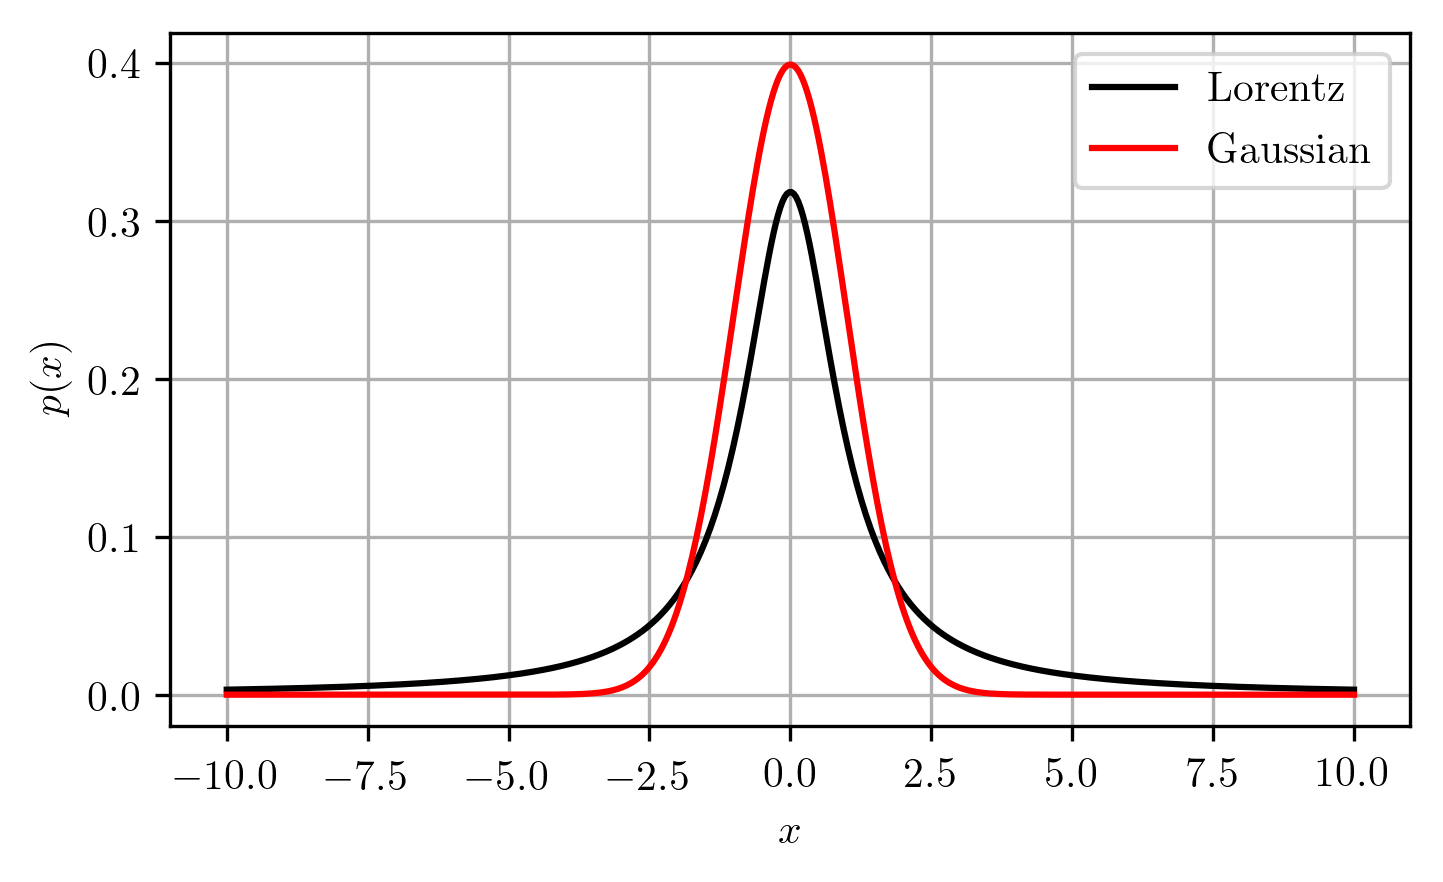
\includegraphics[width=0.75\linewidth]{lorentz.png}
	\caption{Comparison of Lorentzian and Gaussian distributions.}
	\label{fig:compare}
\end{figure}

This shows that for the same set of parameters, the Gaussian has a higher peak, and quickly falls off and approaches zero as one moves away from the mean/central value.

\item Calculate the first moment of the Lorentz distribution assuming that $a = 0$ and $\gamma = 1$.

The first moment of the Lorentzian is given by

\begin{align}
	\ev{x^1} &= \int_{-\infty}^{+\infty} xp(x) \dd{x} \\
	&= \frac{1}{\pi} \int_{-\infty}^{+\infty} \frac{x}{x^2 + 1} \dd{x} \nonumber
\end{align}

Let $u \equiv x^2 + 1$, $\dd{u} \equiv 2x\dd{x}$,

\begin{align}
	\ev{x^1} &= \frac{1}{2\pi} \int_{-\infty}^{+\infty} \frac{1}{u}\dd{u} \nonumber \\
	&= \frac{1}{2\pi} \eval[\ln(u)|_{-\infty}^{+\infty} \nonumber \\
	&= \frac{1}{2\pi} \eval[\ln(x^2 + 1)|_{-\infty}^{+\infty} \nonumber \\
	&= \infty - \infty \nonumber \\
	\Aboxed{
		\ev{x} &= \mathrm{undefined}
	} \label{eq:answer-b}
\end{align}

\item Does the second moment exist?

\begin{equation}\label{eq:2nd-moment}
	\ev{x^2} = \frac{1}{\pi} \int_{-\infty}^{+\infty} \frac{x^2}{x^2 +1}\dd{x}
\end{equation}

By long division of the integrand,

\begin{center}
	\begin{tabular}{c|ccc}
		&&& 1 \\ \cline{2-4}
		$x^2 + 1$ & $x^2$ & $+0x+$ & $0$ \\
		& $x^2$ & $+0x+$ & $1$ \\ \cline{2-4}
		&&& $-1$
	\end{tabular}
\end{center}

From this, \eqref{eq:2nd-moment} can be rewritten as

\begin{align*}
	\ev{x^2} &= \frac{1}{\pi} \int_{-\infty}^{+\infty} 1 - \frac{1}{x^2 + 1} \dd{x} \\
	&= \frac{1}{\pi}\qty[\int_{-\infty}^{+\infty} \dd{x} - \int_{-\infty}^{+\infty} \frac{\dd{x}}{x^2 + 1}]
\end{align*}

The second term is an even function about zero, and can be rewritten as

\begin{align}
	\ev{x^2} &= \frac{1}{\pi}\qty[\int_{-\infty}^{+\infty} \dd{x} - 2\int_0^{+\infty} \frac{\dd{x}}{x^2 + 1}] \nonumber \\
	&= \frac{1}{\pi}\qty[\int_{-\infty}^{+\infty} \dd{x} - 2\eval{\arctan(x)}_0^\infty] \nonumber \\
	&= \frac{1}{\pi}\qty[\int_{-\infty}^{+\infty} \dd{x} - 2\qty(\arctan(\infty) - \arctan(0))] \nonumber \\
	&= \frac{1}{\pi}\qty[\int_{-\infty}^{+\infty} \dd{x} - 2\qty(\frac{\pi}{2} - 0)] \nonumber \\
	&= \frac{1}{\pi}\qty[\int_{-\infty}^{+\infty} \dd{x} - \pi] \nonumber \\
	&= \frac{1}{\pi} \qty[\infty - \pi] \nonumber \\
	\Aboxed{
		\ev{x^2} &= \infty
	} \label{eq:answer-c}
\end{align}

The second moment of the Lorentz distribution exists and has a value of infinity.

\end{enumerate}

\section{P34 PS07 3.45 Central limit theorem}
Use Program \texttt{CentralLimitTheorem} to test the applicability of the central limit theorem.

\begin{enumerate}[(a)]

\item Assume that the variable $s_i$ is uniformly distributed between 0 and 1. Calculate analytically the mean and standard deviation of $s$ and compare your numerical results with your analytical calculation.

The uniform distribution is given by

\begin{equation}\label{eq:uniform}
	p(s) = \frac{1}{b-a}
\end{equation}

where $a$ and $b$ are the bounds of concern. For a variable $s_i$ uniformly distributed $\in [0,1]$, the mean can be obtained by calculating the first moment of \eqref{eq:uniform}:

\begin{align}
	\bar{s} = \ev{s^1} &= \int_0^1 s \dd{s} \\
	&= \eval{\frac{1}{2}s^2}_0^1 \nonumber \\
	\Aboxed{
		\ev{s} &= \frac{1}{2} \label{eq:answer-a-mean}
	}
\end{align}

The standard deviation can be obtained by calculating the square root of the difference of the second moment and the square of the first moment:

\begin{align}
	\sigma &= \sqrt{\ev{s^2} - \ev{s}^2} \label{eq:variance} \\
	\ev{s^2} &= \int_0^1 s^2 \dd{s} \\
	&= \eval{\frac{1}{3}s^2}_0^1 \nonumber \\
	&= \frac{1}{3} \\
	\sigma &= \sqrt{\frac{1}{3} - \qty(\frac{1}{2})^2} \nonumber \\
	&= \sqrt{\frac{1}{12}} \nonumber \\
	\Aboxed{
		\sigma &= \frac{1}{\sqrt{12}} \approx 0.29
	} \label{eq:answer-a-sd}
\end{align}

\item Use the default value of $N = 12$, the number of terms in the sum, and describe the qualitative form of $p(S)$, where $p(S)\Delta S$ is the probability that the sum $S$ is between $S$ and $S +\Delta S$. Does the qualitative form of $p(S)$ change as the number of measurements (trials) of $S$ is increased for a given value of $N$?

As the number of measurements $S$ is increased, the standard deviation $\sigma$ becomes smaller and the expectation value becomes more defined, i.e.

\begin{equation}\label{eq:answer-b}
	\boxed{
		\lim_{S \rightarrow \infty} p(S) = \delta (S)
	}
\end{equation}

\item What is the approximate width of $p(S)$ for $N = 12$? Describe the changes, if any, of the width of $p(S)$ as $N$ is increased. Increase $N$ by at least a factor of 4. Do your results depend strongly
on the number of measurements?

For $N = 12$, running the program \texttt{CentralLimitTheorem} for 40,000 trials yields a variance $\sigma^2 = 0.007$. Its width can be obtained by doubling the standard deviation, given by $\sqrt{\sigma^2}$. Thus, the $\boxed{\mathrm{width} = 1.6}$.

\item To determine the generality of your results, consider the probability density $f(s) = e^{-s}$ for $s \geq 0$ and answer the same questions as in parts (a)-(c).

Its mean is calculated as 

\begin{equation}
	\ev{s} = \int_0^\infty se^{-s} \dd{s} \\
\end{equation}

which can be evaluated using integration by parts. Let $u \equiv s$ and $\dd{v} \equiv e^{-s} \dd{s}$. Consequently, $\dd{u} \equiv \dd{s}$ and $v \equiv -e^{-s}$. We have

\begin{align}
	\ev{s} &= \eval{-se^{-s}}_0^\infty + \int_0^\infty e^{-s} \dd{s} \\
	&= \eval[-se^{-s} - e^{-s} |_0^\infty \nonumber
\end{align}

Since $\dv[2]{s}s < \dv[2]{s}e^{-s}$, the exponential term dominates. Thus,

\begin{align}
	\ev{s} &= 0\cdot e^0 + e^0 \nonumber \\
	\Aboxed{
		\ev{s} &= 1
	} \label{eq:answer-d-mean}
\end{align}

Using $N = 12$, the distribution appears similar to a Poisson distribution. As the number of trials $S$ is increased, the distribution first approaches that of a Gaussian, then of a Dirac delta, similar to \eqref{eq:answer-b}.

Running the program once again for $N=12$ and 40,000 trials, we have $\sigma^2 = 0.021$, which corresponds to a $\boxed{\mathrm{width} = 0.3}$.

\item Consider the Lorentz distribution $f(s) = (1/\pi)(1/(s^2 + 1)$, where $-\infty \leq s \leq \infty$. What is the mean value and variance of $s$? Is the form of $p(S)$ consistent with the results that you found in parts (b)–(d)?

Its mean value is

\begin{equation}
	\ev{s} = \frac{1}{\pi} \int_{-\infty}^{+\infty} \frac{s}{s^2 +1} \dd{s}
\end{equation}

Let $u \equiv s^2 + 1$, $\dd{u} \equiv 2s\dd{s}$,

\begin{align}
	\ev{s} &= \frac{1}{2\pi} \int_{-\infty}^{+\infty} \frac{\dd{u}}{u} \nonumber \\
	&= \frac{1}{2\pi} \eval{\ln u}_{-\infty}^{+\infty} \nonumber \\
	\Aboxed{
		\ev{s} &= \mathrm{undefined}
	} \label{eq:answer-e-mean}
\end{align}

From \eqref{eq:variance}, we know that the variance is dependent on the mean. Consequently, the variance of $s$ is undefined.

\item Each value of $S$ can be considered to be a measurement. The sample variance $\tilde{\sigma}_S^2$ is a measure of the square of the differences of the result of each measurement and is given by

\begin{equation}
	\tilde{\sigma}_S^2 = \frac{1}{N-1}\sum_{i=1}^N (S_i - \bar{S})^2
\end{equation}

The reason for the factor of $N-1$ rather than $N$ in the definition of $\tilde{\sigma}_S^2$ is that to compute it, we need to use the $N$ values of $s$ to compute the mean of $S$, and thus, loosely speaking, we have only $N-1$ independent values of $s$ remaining to calculate $\tilde{\sigma}_S^2$. Show that if $N \gg 1$, then
$\tilde{\sigma}_S^2 \approx \sigma_S$, where the standard deviation $\sigma_S$ is given by $\sigma_S^2 = \overline{S^2} - \overline{S}^2$.

With $N \gg 1$, we can drop the $-1$ term in the denominator since its contribution becomes negligible:

\begin{equation}
	\tilde{\sigma}_S^2 = \frac{1}{N}\sum_{i=1}^N (S_i - \bar{S})^2
\end{equation}

Expanding the summation and simplifying,'

\begin{align}
	\tilde{\sigma}_S^2 &\approx \frac{1}{N}\qty[(S_1 - \bar{S})^2 + (S_2 - \bar{S})^2 + \hdots + (S_N - \bar{S})^2] \nonumber \\
	&\approx \frac{1}{N}\qty[S_1^2 - 2S_1\bar{S}^2 + S_2^2 - 2S_2\bar{S}^2 + \hdots + S_N^2 - 2S_N\bar{S} + \bar{S}^2] \nonumber \\
	&\approx \frac{1}{N} [(S_1^2 + S_2^2 + \hdots + S_N^2) \nonumber \\
	&\quad - 2\bar{S}(S_1 + S_2 + \hdots + S_N) + N\bar{S}^2] \nonumber \\
	&\approx \frac{S_1^2 + S_2^2 + \hdots + S_N^2}{N} - 2\bar{S}\frac{S_1 + S_2 + \hdots + S_N}{N} + \bar{S}^2 \nonumber \\
	&\approx \bar{S^2} - 2\bar{SS} + \bar{S}^2 = \bar{S^2} - 2\bar{S}^2 + \bar{S}^2 \\
	&\approx \bar{S^2} - \bar{S}^2 = \sigma_S^2
\end{align}

Take the square root of both sides,

\begin{equation}
	\boxed{
		\tilde{\sigma}_S \approx \sigma_S
	}
\end{equation}

\item The quantity $\tilde{\sigma}_S$ is known as the standard deviation of the means. That is, $\tilde{\sigma}_S$ is a measure of how much variation we expect to find if we make repeated measurements of $S$. How does the value of $\tilde{\sigma}_S$ compare to your estimated width of the probability density $p(S)$?

\begin{align}
	\tilde{\sigma}_S^2 &= \frac{1}{N-1}\sum_{i=1}^N (S_i - \bar{S})^2 \cdot \frac{N}{N} \\
	&= \frac{N}{N - 1}\sigma_S^2
\end{align}

Using the variance $\sigma_S^2 = 1/12$ for a uniform distribution, solve for $\sigma_S^2$ given varying values of $N$. For $N=12$, 

\begin{align}
	\tilde{\sigma}_S^2(N=12) &= \frac{12}{12-1}\frac{1}{12} \\
	&= \frac{1}{11} \\
	&\approx 0.1
\end{align}

Then the value of $\tilde{\sigma}_S$ is

\begin{equation}
	\tilde{\sigma}_S(N=12) = \sqrt{\frac{1}{11}} \approx 0.3
\end{equation}

The approximated width is lower than that of $\tilde{\sigma}_S$ for $N=12$.

\end{enumerate}

\section{P35 PS07 3.72 Alternative derivation of the Gaussian distribution}
On page 138 we evaluated the binomial probability $P_N(n)$ using Stirling’s approximation to determine the parameters $A$, $B$, and $\tilde{n}$ in (3.109). Another way to determine these parameters is to
approximate the binomial distribution by a Gaussian and require that the zeroth, first, and second moments of the Gaussian and binomial distribution be equal. We write

\begin{equation}
	P(n) = Ae^{-B(n - \tilde{n})^2/2}
\end{equation}

where $A$, $B$, and $\tilde{n}$ are the parameters to be determined. We first require that

\begin{equation}
	\int_0^N P(n) \dd{n} = 1
\end{equation}

Because $P(n)$ depends on the difference $n-\tilde{n}$, it is convenient to change the variable of integration in (3.196) to $x = n - \tilde{n}$ and write

\begin{equation}
	\int_{-Np}^{N(1-p)} P(x)\dd{x} = 1
\end{equation}

where

\begin{equation}
	P(x) = Ae^{-Bx^2/2} \label{eq:3.72-changevar}
\end{equation}

Because we are interested in the limit $N \rightarrow \infty$, we can extend the limits in (3.197) to $\pm \infty$:

\begin{equation}
	\int_{-\infty}^{\infty} P(x)\dd{x} = 1 \label{eq:3.72-normcondition}
\end{equation}

\begin{enumerate}[(a)]

\item The first moment of the Gaussian distribution is

\begin{equation}
	\bar{n} = \int_{-\infty}^\infty nP(n) \dd{n}
\end{equation}

where $P(n)$ is given by (3.195). Make a change of variables and show that

\begin{equation}
	\bar{n} = \int_{-\infty}^\infty (x+\tilde{n})P(x)\dd{x} = \tilde{n} \label{eq:3.72-given}
\end{equation}

Using \eqref{eq:3.72-normcondition} to solve $A$ in terms of $B$,

\begin{align}
	1 &= \int_{-\infty}^\infty Ae^{-Bx^2/2} \dd{x} \\
	&= A\int_{-\infty}^\infty e^{-Bx^2/2} \dd{x} \\
	&= A\sqrt{\frac{2\pi}{B}}
\end{align}

such that

\begin{equation}
	A = \sqrt{\frac{B}{2\pi}}
\end{equation}

\eqref{eq:3.72-changevar} can now be rewritten as

\begin{equation}
	P(x) = \sqrt{\frac{B}{2\pi}} e^{-Bx^2/2} \label{eq:3.72-recast}
\end{equation}

Substituting the above into \eqref{eq:3.72-given},

\begin{align}
	\bar{n} &= \int_{-\infty}^\infty (x+\tilde{n})\sqrt{\frac{B}{2\pi}} e^{-Bx^2/2} \dd{x} \\
	&= \sqrt{\frac{B}{2\pi}}\qty(\int_{-\infty}^\infty xe^{-Bx^2/2}\dd{x} + \tilde{n} \int_{-\infty}^\infty e^{-Bx^2/2}\dd{x}) \nonumber
\end{align}

According to A.16,

\begin{equation}
	\int_{-\infty}^\infty ue^{-au^2} \dd{u} = 0
\end{equation}

which means the first integral is zero. The second integral is similar to an earlier one. Simplifying,

\begin{align}
	\bar{n} &= \sqrt{\frac{B}{2\pi}}\qty(0 + \tilde{n}\frac{2\pi}{B}) \\
	&= \sqrt{\frac{B}{2\pi}}\tilde{n}\sqrt{\frac{2\pi}{B}} \\
	\Aboxed{
		\bar{n} &= \tilde{n}
	} \qed
\end{align}

\item The first moment of the binomial distribution is given by $pN$ according to (3.96). Require the first moments of the binomial and Gaussian distributions to be equal, and determine $\tilde{n}$.

The first moment of the binomial distribution is

\begin{equation}
	\bar{n}_{binom} = pN
\end{equation}

The first moment of the Gaussian distribution is

\begin{equation}
	\bar{n}_{gauss} = \tilde{n}
\end{equation}

Requiring the two to be equal gives

\begin{equation}
	\boxed{
		\tilde{n} = pN
	}
\end{equation}

\item The variance of the binomial distribution is given in (3.99) and is equal to $\overline{(n - \bar{n})^2} = Npq$. The corresponding variance of the Gaussian distribution is given by

\begin{equation}
	\overline{(n - \bar{n})^2} = \int_{-\infty}^\infty (n - \bar{n})^2 P(n) \dd{n}
\end{equation}

Make the necessary change of variables in (3.202) and do the integrals in (3.199) and (3.202) [see (A.23) and (A.17)] to confirm that the values of $B$ and $A$ are given by (3.115) and (3.117), respectively.

Let $x \equiv n - \tilde{n}$, $n \equiv x+\tilde{n}$, $\bar{n} = \tilde{n}$. Substituting in,

\begin{align}
	\overline{(n - \bar{n})^2} &= \int_{-\infty}^\infty (x+\tilde{n}-\tilde{n})^2 P(x)\dd{x} \\
	&= \int_{-\infty}^\infty x^2 P(x)\dd{x} \\
	&= \int_{-\infty}^\infty x^2 \sqrt{\frac{B}{2\pi}}e^{-Bx^2/2\dd{x}} \\
	&= \sqrt{\frac{B}{2\pi}} \int_{-\infty}^\infty x^2 e^{-Bx^2/2}\dd{x}
\end{align}

From A.17,

\begin{equation}
	\int_{-\infty}^\infty x^2 e^{-ax^2}\dd{x} = \frac{1}{2}\qty(\frac{\pi}{a^3})^{\frac{1}{2}}
\end{equation}

We have

\begin{align}
	\overline{(n - \bar{n})^2} &= \sqrt{\frac{B}{2\pi}} \frac{1}{2} \qty(\frac{8\pi}{B^3})^{\frac{1}{2}} \\
	&= \sqrt{\frac{1}{B}}\sqrt{\frac{2\pi}{B}} \\
	&= \frac{1}{B}
\end{align}

The variance of the binomial distribution is given by

\begin{equation}
	\overline{(n - \bar{n})^2}_{binom} = Npq
\end{equation}

Since it was stated that the first and second moments of the Gaussian and binomial distributions are equal, then their variances must also be equal. Then,

\begin{align}
	\Aboxed{
		B &= \frac{1}{Npq}
	} \\
	\Aboxed{
		A &= \sqrt{\frac{1}{2\pi Npq}} 
	}
\end{align}

\item Explain why the third moments of the binomial and Gaussian distribution are not equal.

The third moment is a measure of the asymmetricity of a probability distribution about its mean value. This means that a symmetric probability distribution has a zero third moment. The Gaussian is always symmetric about its mean, while the binomial distribution is not always so. Hence, their third moments are not equal.

\end{enumerate}

\section{P36 PS08 4.5 Standard deviation of the energy of subsystem $A$}
Use the results of Table \ref{tab:4.5-given} to find the standard deviation of the energy of subsystem $A$.

\begin{table}[h!]
	\centering
	\begin{tabular}{|c|c||c|c|c|}
		\hline
		$E_A$ & $\Omega_A(E_A)$ & $\Omega_B(6-E_A)$ & $\Omega_A\Omega_B$ & $P_A(E_A)$ \\ \hline
		6 & 7 & 1 & 7 & 7/84 \\ \hline
		5 & 6 & 2 & 12 & 12/84 \\ \hline
		4 & 5 & 3 & 15 & 15/84 \\ \hline
		3 & 4 & 4 & 16 & 16/84 \\ \hline
		2 & 3 & 5 & 15 & 15/84 \\ \hline
		1 & 2 & 6 & 12 & 12/84 \\ \hline
		0 & 1 & 7 & 7 & 7/84 \\ \hline
	\end{tabular}
	\caption{The probability $P_A(E_A)$ that subsystem $A$ has energy $E_A$ given $N_A = N_B = 2$ and $E_{tot} = E_A + E_B = 6$.}
	\label{tab:4.5-given}
\end{table}

The standard deviation of the energy of subsystem $A$ is given by

\begin{equation}
	\sigma = \sqrt{\ev{E_A^2} - \ev{E_A}^2} \label{eq:sd}
\end{equation}

The first moment (mean) $\ev{E_A}$ is obtained by

\begin{align}
	\ev{E_A} &= \sum_{i=1}^N (E_A)_i (P_A)_i \label{eq:mean} \\
	&= 6\qty(\frac{7}{84}) + 5\qty(\frac{12}{84}) + 4\qty(\frac{15}{84}) \nonumber \\
	&+ 3\qty(\frac{16}{84}) + 2\qty(\frac{15}{84}) + 1\qty(\frac{12}{84}) + 0\qty(\frac{7}{84}) \nonumber \\
	&= 12 \nonumber
\end{align}

The second moment (raw variance) $\ev{E_A^2}$ is obtained by

\begin{align}
	\ev{E_A^2} &= \sum_{i=1}^N (E_A)_i^2 (P_A)_i \label{eq:var} \\
	&= 36\qty(\frac{7}{84}) + 25\qty(\frac{12}{84}) + 16\qty(\frac{15}{84}) \nonumber \\
	&+ 9\qty(\frac{16}{84}) + 4\qty(\frac{15}{84}) + 1\qty(\frac{12}{84}) + 0\qty(\frac{7}{84}) \nonumber \\
	&= 3 \nonumber
\end{align}

So the standard deviation is

\begin{align}
	\sigma &= \sqrt{12 - 3^2} \nonumber \\
	&= \sqrt{3} \nonumber \\
	\Aboxed{
		\sigma &\approx 1.73
	}
\end{align}

\section{P37 PS08 4.10 Rapid increase in the number of states}

\begin{enumerate}[(a)]

\item Consider an Einstein solid of $N = 20$ distinguishable particles. What is the total number of accessible microstates $\Omega (E)$ for $E = 10, 102, 103, \hdots$? Is $\Omega (E)$ a rapidly increasing function of $E$ for fixed $N$?

For an Einstein solid of $N=20$ distinguishable particles, the total number of accessible microstates $\Omega(E)$ is given by

\begin{equation}
	\Omega(E) = \frac{\qty(E + N - 1)!}{E!\qty(N-1)!} \label{eq:accessible}
\end{equation}

For various $E$, we have

\begin{align}
	\Omega(E = 10) &= \frac{\qty(10 + 20 - 1)!}{10!\qty(20-1)!} \nonumber \\
	\Aboxed{
		\Omega(E = 10) &= 20,030,010
	} \\
	\Omega(E=100) &= \frac{\qty(100 + 20 - 1)!}{100!\qty(20-1)!} \nonumber \\
	\Aboxed{
		\Omega(E = 100) &\approx 4.91 \times 10^{21}
	} \\
	\Omega(E=1000) &= \frac{\qty(1000 + 20 - 1)!}{1000!\qty(20-1)!} \nonumber \\
	\Aboxed{
		\Omega(E = 1000) &\approx 9.93 \times 10^{39}
	} 
\end{align}

Continuing this process for larger $E$ for fixed $N$, we obtain the graph in Figure \ref{fig:microstates}.

\begin{figure}[h!]
	\centering
	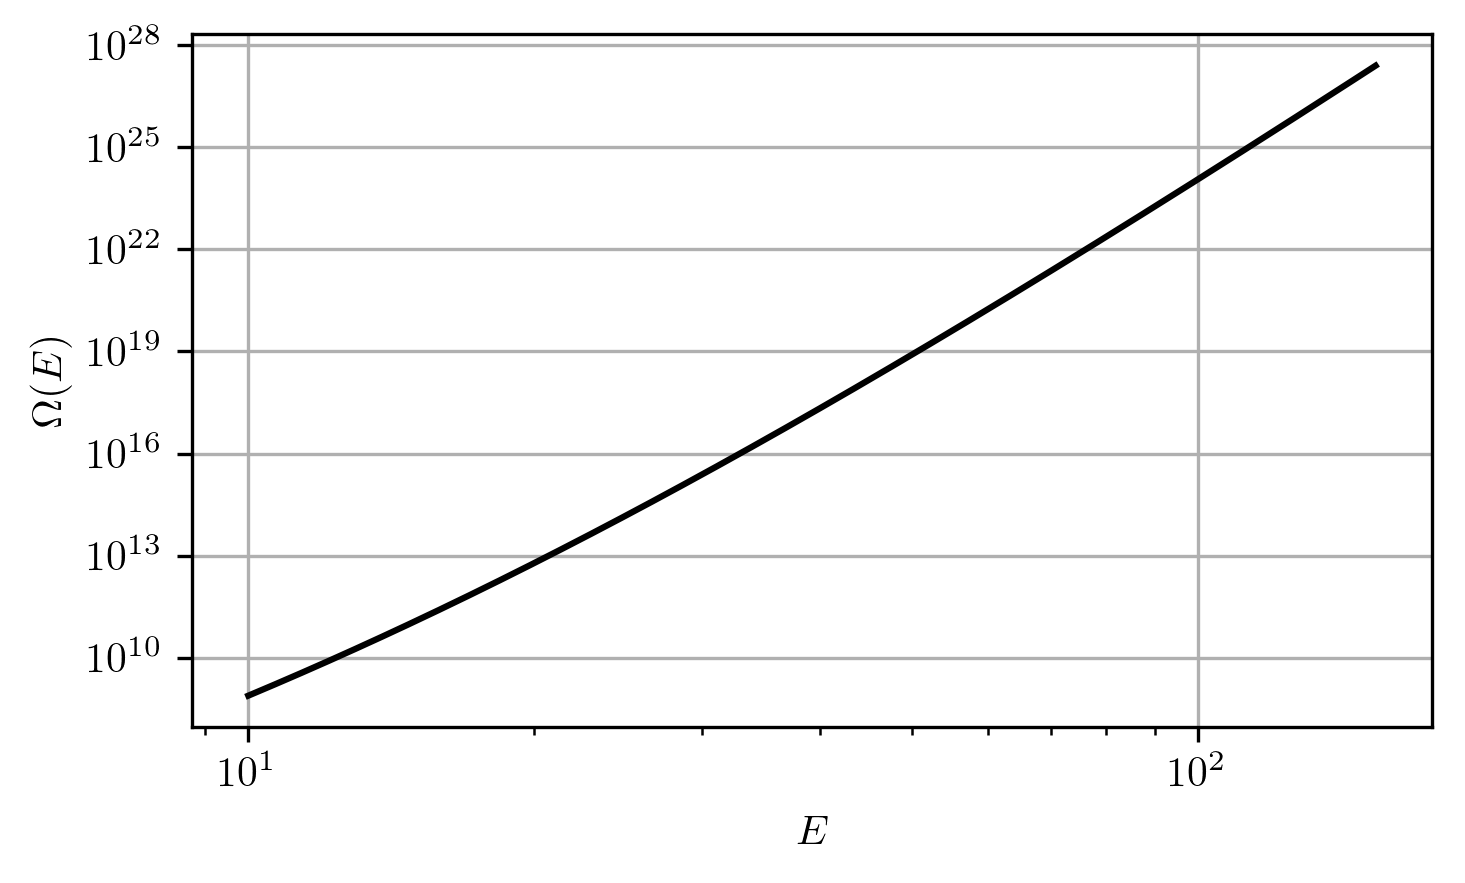
\includegraphics[width=0.75\linewidth]{microstates.png}
	\caption{$\Omega(E) \forall E \in \qty[10^1, 10^3]$}
	\label{fig:microstates}
\end{figure}

Thus, $\Omega(E)$ is an exponentially increasing function of $E$ for fixed $N$.

\item Is $\Omega$ rapidly increasing function of $N$ for fixed $E$?

For fixed $E = 10$ and varying $N$, we obtain the graph in Figure \ref{fig:fixed-N}.

\begin{figure}[h!]
	\centering
	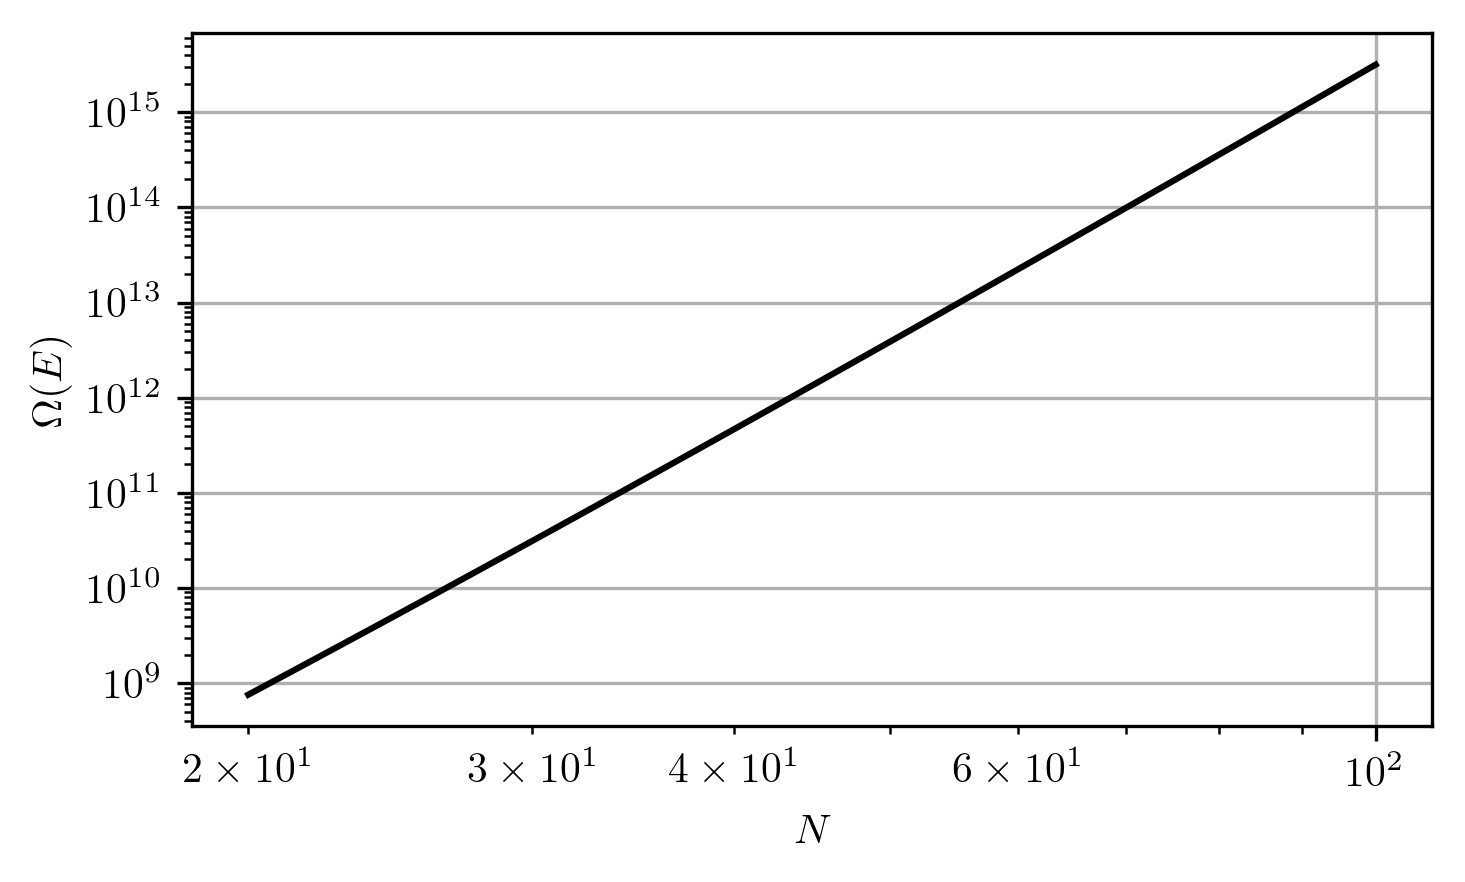
\includegraphics[width=0.75\linewidth]{fixedN.png}
	\caption{$\Omega(E) \forall N \in \qty[20, 100]$}
	\label{fig:fixed-N}
\end{figure}

Thus, $\Omega(E)$ is also an exponentially increasing function of $N$ for fixed $E$.

\end{enumerate}

\section{P38 PS08 4.14 Estimation of number of states}
Estimate the number of microstates accessible to a gas molecule in a one liter box at room temperature. The mean energy $E$ of a gas molecule such as nitrogen at room temperature can be found from the relation $E = 3kT/2$. Consider an energy interval $\Delta E = 10^{-27}$ J that is much smaller than $E$, and calculate the number of microstates $g(E)\Delta E$ accessible to the molecule in the interval between $E$ and $E + \Delta E$. Refer to (4.42) and (4.17).

From GT 4.42, the number of microstates accessible to a gas molecule in a 1-liter box is

\begin{equation}
	\Gamma(E) = \frac{4\pi}{3}\frac{V}{h^3}\qty(2mE)^{3/2} \label{eq:given-states}
\end{equation}

and from GT 4.17, the number of microstates in the energy interval $\qty[E, E+\Delta E]$ is

\begin{equation}
	g(E)\Delta E = \Gamma(E+\Delta E) - \Gamma(E) \approx \dv{\Gamma(E)}{E}\Delta E \label{eq:given-interval}
\end{equation}

The mean energy of a gas molecule is given by

\begin{equation}
	E = \frac{3}{2}kT \label{eq:mean-energy}
\end{equation}

If we consider room temperature to be $T = 25^\circ C = 298 K$, then \eqref{eq:mean-energy} becomes

\begin{align}
	E &= \frac{3}{2}\qty(1.38\times 10^{-23} \mathrm{m^2\cdot kg\cdot s^{-2}\cdot K^{-1}})\qty(298 \mathrm{K}) \nonumber \\
	&\approx 6.17\times 10^{-21} \mathrm{J} \label{eq:answer-energy}
\end{align}

We consider diatomic nitrogen since it comprises around 3/4 of the atmosphere. Its molar mass is 28.02 g$\cdot$mol$^{-1}$. The mass for a nitrogen molecule is then given by

\begin{align}
	m &= \frac{\nu}{N_A} \nonumber \\
	&= \frac{28.02\mathrm{g}}{6.022\times 10^{23}} \nonumber \\
	&= 4.65\times 10^{-26} \mathrm{kg} \label{eq:answer-mass}
\end{align}

From \eqref{eq:given-interval}, we differentiate \eqref{eq:given-states} w.r.t. $E$:

\begin{align}
	\dv{\Gamma(E)}{E}\Delta E &= \frac{4\pi V}{3h^3}\qty(2m)^{3/2} \frac{3}{2}E^{1/2} \Delta E \nonumber \\
	&= \frac{2\pi V}{h^3}\qty(2m)^{3/2}\sqrt{E}\Delta E \nonumber
\end{align}

If we consider an energy interval $\Delta E = 10^{-27}$ J, this becomes

\begin{equation}
	g(E)\Delta E = \frac{2\pi\qty(1\mathrm{ L})\qty[2\qty(4.65\times 10^{-26}\mathrm{ kg})]^{3/2}\sqrt{6.17\times 10^{-21}\mathrm{ J}}}{\qty(6.63\times 10^{-34}\mathrm{ m^2\cdot kg\cdot s^{-1}})^3}\qty(10^{-27}\mathrm{ J}) \nonumber
\end{equation}

\begin{equation}
	\boxed{
		g(E)\Delta E \approx 4.80\times 10^{22}
	} \label{eq:answer}
\end{equation}

\section{P39 PS08 4.15 Approximate expression for $\Gamma(E,V,N)$}
We can obtain an approximate expression for $\Gamma(E, V,N)$ using simpler physical considerations. We write

\begin{align}
	\Gamma(E,V,N) &\approx \frac{1}{N!}\Gamma_1\qty(\frac{E}{N},V)\Gamma_1\qty(\frac{E}{N},V) \hdots \Gamma_1\qty(\frac{E}{N},V) \nonumber \\
	&\approx \frac{1}{N!}\Gamma_1\qty(\frac{E}{N},V)^N
\end{align}

where $\Gamma_1(E, V)$ is the number of states of a single particle with energy less than $E$ in a three-dimensional box of volume $V$. We have assumed that on the average each particle has an energy $E/N$. Find the form of $\Gamma(E, V,N)$ using the relation (4.42) for $\Gamma_1$. How does the dependence on $V$ and $E$ of $\Gamma(E, V,N)$ obtained from this simple argument compare to the $V$ and $E$ dependence of $\Gamma$ in (4.49). What about the $N$ dependence?

Given the following:

\begin{eqnarray}
	\Gamma(E,V,N) \approx \frac{1}{N!}\Gamma_1\qty(\frac{E}{N}, V)^N \label{eq:4.15-given1} \\
	\Gamma_1(E) = \frac{4\pi V}{3h^3}\qty(2mE)^{3/2} \label{eq:4.15-given2}
\end{eqnarray}

We wish to find the form of $\Gamma(E,V,N)$ for $\Gamma_1$. \eqref{eq:4.15-given2} becomes

\begin{equation}
	\Gamma_1\qty(\frac{E}{N}) = \frac{4\pi V}{3h^3}\qty(\frac{2mE}{N})^{3/2}
\end{equation}

Plugging this into \eqref{eq:4.15-given1}, we have

\begin{align}
	\Gamma(E,V,N) &= \frac{1}{N!}\qty[\frac{4\pi V}{3h^3}\qty(\frac{2mE}{N})^{3/2}]^N \nonumber \\
	\Aboxed{
		\Gamma(E,V,N) &= \frac{1}{N!}\qty(\frac{4\pi V}{3h^3})^N \qty(\frac{2mE}{N})^{3N/2}
	} \label{eq:4.15-answer}
\end{align}

From \eqref{eq:4.15-answer}, we see that $\Gamma \propto V^N$, $\Gamma \propto E^{3N/2}$, and $\Gamma \propto \qty(N!N^{3N/2})^{-1}$. In contrast, the form of $\Gamma(E,V,N)$ given in GT 4.49 is

\begin{equation}
	\Gamma(E,V,N) = \frac{1}{N!}\qty(\frac{V}{h^3})^N \frac{\qty(2\pi mE)^{3N/2}}{\qty(3N/2)!} \label{eq:4.15-semiclassical}
\end{equation}

where $\Gamma \propto V^N$, $\Gamma \propto E^{3N/2}$, and $\Gamma \propto \qty[N!\qty(3N/2)!]^{-3N/2}$.

\section{P40 PS08 4.16 Density of states of ideal gas}
Use (4.51) to calculate the density of states $g(E, V,N)$ and verify that $\Gamma(E, V,N)$ and $g(E, V,N)$ are rapidly increasing functions of $E$, $V$ , and $N$.

Given the following:

\begin{equation}
	\ln \Gamma(E,V,N) = N \ln\frac{V}{N} + \frac{3}{2}N\ln\frac{mE}{3N\pi\hbar^2} + \frac{5}{2}N \label{eq:4.16-given}
\end{equation}

The density of states is given by

\begin{equation}
	g(E,V,N) \approx \dv{\Gamma(E)}{E} \label{eq:4.16-density-states}
\end{equation}

We take the exponential of both sides of \eqref{eq:4.16-given}:

\begin{align}
	\ln\Gamma(E,V,N) &= \ln(\frac{V}{N})^N + \ln(\frac{mE}{3N\pi\hbar^2})^{3N/2} + \frac{5}{2}N \nonumber \\
	\ln\Gamma(E,V,N) &= \ln\qty[\qty(\frac{V}{N})^N \qty(\frac{mE}{3N\pi\hbar^2})^{3N/2}] + \frac{5}{2}N \nonumber \\
	\Gamma(E,V,N) &= \qty(\frac{V}{N})^N \qty(\frac{mE}{3N\pi\hbar^2})^{3N/2} e^{5N/2} \label{eq:4.16-gamma}
\end{align}

Since $\Gamma \propto V^N$, $\Gamma \propto N^{-5N/2}e^{5N/2}$, and $\Gamma \propto E^{3N/2}$, $\Gamma$ is a rapidly increasing function of $E$ and $V$. Note that because $\dd[2]_N\qty(e^{5N/2}) > \dd[2]_N\qty(N^{-5N/2})$, the exponential term dominates and thus, $\Gamma$ is also a rapidly increasing function of $N$.

From \eqref{eq:density-states}, we differentiate \eqref{eq:4.16-gamma} w.r.t. $E$:

\begin{equation}
	\boxed{
		g(E,V,N) = \qty(\frac{V}{N})^N \qty(\frac{m}{3N\pi\hbar^2})^{3N/2} e^{5N/2} \frac{3N}{2} E^{N/2}
	} \label{eq:4.16-answer}
\end{equation}

Now, $g \propto V^N$, $g \propto e^{5N/2}$, and $g \propto E^{N/2}$, so $g$ is also a rapidly increasing function of $E$, $V$, and $N$.

\section{P41 PS08 4.19 The Sackur-Tetrode expression for the entropy}
Use the relations (4.63) and (4.65) to obtain $S$ as a function of $T$, $V$, and $N$ instead of $E$, $V$, and $N$. This relation is known as the Sackur-Tetrode equation.

Given the following:

\begin{align}
	S(E,V,N) &= Nk\qty[\ln\frac{V}{N} + \frac{3}{2}\ln\qty(\frac{mE}{3N\pi\hbar^2}) + \frac{5}{2}] \label{eq:4.19-given-s} \\
	E &= \frac{3}{2}NkT \label{eq:4.19-given-e}
\end{align}

Substitute \eqref{eq:4.19-given-e} in \eqref{eq:4.19-given-s}:

\begin{align}
	S &= Nk\qty[\ln\frac{V}{N} + \frac{3}{2}\ln\qty(\frac{m}{3N\pi\hbar^2} \frac{3}{2}NkT) + \frac{5}{2}] \\
	&= Nk\qty[\ln\frac{V}{N} + \frac{3}{2}\ln\qty(\frac{mkT}{2\pi\hbar^2}) + \frac{5}{2}]
\end{align}

Rewrite in terms of $h \equiv 2\pi\hbar$:

\begin{align}
	S &= Nk\qty[\ln\frac{V}{N} + \frac{3}{2}\ln\qty(\frac{4\pi^2 mkT}{2\pi h^2}) + \frac{5}{2}] \\
	&= Nk\qty[\ln\frac{V}{N} + \frac{3}{2}\ln\qty(\frac{2\pi mkT}{h^2}) + \frac{5}{2}] \\
	&= Nk\qty[\ln\qty(\frac{V}{N}\qty(\frac{2\pi mkT}{h^2})^{3/2}) + \frac{5}{2}] \\
	\Aboxed{
		\frac{S}{Nk} &= \ln\qty[\frac{V}{N}\qty(\frac{2\pi mkT}{h^2})^{3/2}] + \frac{5}{2}
	}
\end{align}

which is the Sackur-Tetrode relation.

\section{P42 PS08 4.20 Chemical potential of an ideal gas}
Use (4.61) and (4.63) to derive the dependence of the chemical potential $\mu$ on $E$, $V$, and $N$ for an ideal classical gas. Then use (4.65) to determine $\mu(T, V,N)$. We will derive $\mu(T, V,N)$ for the ideal classical gas more simply in Section 6.6.

Given the following:

\begin{align}
	\frac{\mu}{T} &= -\qty(\pdv{S}{N})_{E,V} \label{eq:4.20-given-mu} \\
	S(E,V,N) &= Nk\qty[\ln\frac{V}{N} + \frac{3}{2}\ln\qty(\frac{mE}{3N\pi\hbar^2}) + \frac{5}{2}] \label{eq:4.20-given-s} \\
	E &= \frac{3}{2}NkT \label{eq:4.20-given-e}
\end{align}

Perform the necessary differentiation on \eqref{eq:4.20-given-s} according to \eqref{eq:4.20-given-mu} and simplify:

\begin{align}
	\frac{\mu}{T} &= -\pdv{N} \qty{Nk\qty[\ln\frac{V}{N} + \frac{3}{2}\ln\qty(\frac{mE}{3N\pi\hbar^2}) + \frac{5}{2}]} \\
	&= -\pdv{N} \qty[kN\ln\frac{V}{N} + \frac{3}{2}kN\ln\qty(\frac{mE}{3N\pi\hbar^2}) + \frac{5}{2}kN] \\
	&= -\qty[-k + k\ln\qty(\frac{V}{N}) - \frac{3}{2}k + \frac{3}{2}k\ln\qty(\frac{mE}{3N\pi\hbar^2}) + \frac{5}{2}k] \\
	&= -k\qty[-1 + \ln\qty(\frac{V}{N}) + \frac{3}{2}\ln\qty(\frac{mE}{3N\pi\hbar^2}) + 1] \\
	&= -k\qty[\ln\qty(\frac{V}{N}) + \frac{3}{2}\ln\qty(\frac{mE}{3N\pi\hbar^2})] \\
	&= -k\ln\qty[\frac{V}{N}\qty(\frac{mE}{3N\pi\hbar^2})^{3/2}] \\
	\Aboxed{
		\mu &= -kT\ln\qty[\frac{V}{N}\qty(\frac{mE}{3N\pi\hbar^2})^{3/2}]
	} \label{eq:4.20-answer-1}
\end{align}

Plugging in \eqref{eq:4.20-given-e},

\begin{align}
	\mu(T,V,N) &= -kT\ln\qty[\frac{V}{N}\qty(\frac{m}{3N\pi\hbar^2}\frac{3}{2}NkT)^{3/2}] \\
	&= -kT\ln\qty[\frac{V}{N}\qty(\frac{mkT}{2\pi\hbar^2})^{3/2}]
\end{align}

Using the relation $h = 2\pi\hbar$, rewrite as

\begin{align}
	\mu(T,V,N) &= -kT\ln\qty[\frac{V}{N}\qty(\frac{4\pi^2 mkT}{2\pi h^2})^{3/2}] \\
	\Aboxed{
		\mu(T,V,N) &= -kT\ln\qty[\frac{V}{N}\qty(\frac{2\pi mkT}{h^2})^{3/2}]
	} \label{eq:4.20-answer-2}
\end{align}

\section{P43 PS08 4.21 The energy as a function of the temperature}
Solve (4.72) for $n/N$ and verify (4.74). Then use (4.14) to solve for $E$ as a function of $T$ and verify (4.73) for a system of $N$ noninteracting spins.

Given the following:

\begin{align}
	\frac{1}{T} &= -k\frac{1}{2\mu B}\ln\qty(\frac{N-n}{n}) \label{eq:4.21-given-t} \\
	E &= -(2n - N)\mu B \label{eq:4.21-given-e}
\end{align}

Solving for $n/N$ in \eqref{eq:4.21-given-t}:

\begin{align}
	-\frac{2\mu B}{kT} &= \ln\qty(\frac{N - n}{n}) \\
	e^{-2\mu B/kT} &= \frac{N-n}{n} \\
	e^{-2\mu B/kT} &= \frac{N}{n} - 1 \\
	1 + e^{-2\mu B/kT} &= \frac{N}{n} \\
	\Aboxed{
		\frac{n}{N} &= \frac{1}{1 + e^{-2\mu B/kT}}
	} \label{eq:4.21-answer-1}
\end{align}

Let $\beta \equiv 1/kT$. With some further manipulation:

\begin{align}
	\frac{n}{N} &= \frac{1}{1 + e^{-2\beta\mu B}} \cdot \frac{e^{\beta\mu B}}{e^{\beta\mu B}} \\
	\Aboxed{
	\frac{n}{N} &= \frac{e^{\beta\mu B}}{e^{\beta\mu B} + e^{-\beta\mu B}}
	} \label{eq:4.21-answer-2}
\end{align}

which is the same form obtained in GT (4.74b). Solving for $n/N$ in \eqref{eq:4.21-given-e}:

\begin{align}
	E &= -(2n - N)\mu B \cdot \frac{N}{N} \\
	&= -\frac{2n - N}{N}N\mu B \\
	&= -\qty(\frac{2n}{N} - 1)N\mu B
\end{align}

Substitute \eqref{eq:4.21-answer-1} into this:

\begin{align}
	E &= -\qty(2\frac{e^{\beta\mu B}}{e^{\beta\mu B} + e^{-\beta\mu B}} - 1)N\mu B \\
	&= -\qty(\frac{2e^{\beta\mu B} - e^{\beta\mu B} - e^{-\beta\mu B} }{e^{\beta\mu B} + e^{-\beta\mu B}})N\mu B \\
	&= -\qty(\frac{e^{\beta\mu B} - e^{-\beta\mu B} }{e^{\beta\mu B} + e^{-\beta\mu B}})N\mu B
\end{align}

which can be simplified using the relation $\tanh(x) \equiv \frac{e^{x} - e^{-x} }{e^{x} + e^{-x}}$:

\begin{align}
	E &= -\tanh(\beta\mu B)N\mu B \\
	\Aboxed{
		E &= -N\mu B\tanh(\frac{\mu B}{kT})
	} \label{eq:4.21-answer-3}
\end{align}

which is the same form as that in GT (4.73).

\section{P44 PS08 4.22 The Einstein solid in the microcanonical ensemble}
Consider a collection of $N$ distinguishable harmonic oscillators with total energy $E$. The oscillators are distinguishable because they are localized on different lattice sites. In one dimension the energy of each particle is given by $\epsilon_n = (n + \frac{1}{2})\hbar\omega$, where $\omega$ is the angular frequency. Hence, the total energy can be written as $E = (Q + \frac{1}{2}N)\hbar\omega$, where $Q$ is the number of quanta. Calculate the dependence of the temperature $T$ on the total energy $E$ in the microcanonical ensemble using the result that the number of accessible microstates in which $N$ distinguishable oscillators can share $Q$ indistinguishable quanta is given by $\Omega = (Q + N - 1)!/Q!(N - 1)!$ [see (4.3)]. Then use this relation to find $E(T)$. This relation is calculated much more simply in the canonical ensemble as shown in Example 4.3.

Given the following:

\begin{equation}
	E = \qty(Q + \frac{1}{2}N)\hbar\omega \label{eq:given-e}
\end{equation}

Solving for $Q$:

\begin{align}
	\frac{E}{\hbar\omega} &= Q + \frac{1}{2}N \\
	Q &= \frac{E}{\hbar\omega} - \frac{1}{2}N \label{eq:inter-q}
\end{align}

The number of accessible microstates in which $N$ distinguishable oscillators can share $Q$ indistinguishable quanta is given by

\begin{equation}
	\Omega = \frac{\qty(Q+N-1)!}{Q!\qty(N-1!)} \label{eq:microstates}
\end{equation}

Substituting \eqref{eq:inter-q} into \eqref{eq:microstates}:

\begin{align}
	\Omega &= \frac{\qty(\frac{E}{\hbar\omega} - \frac{1}{2}N + N - 1)!}{\qty(\frac{E}{\hbar\omega} - \frac{1}{2}N)! \qty(N-1)!} \\
	&= \frac{\qty(\frac{E}{\hbar\omega} + \frac{1}{2}N -1)!}{\qty(\frac{E}{\hbar\omega} - \frac{1}{2}N)!(N-1)!} \label{eq:inter-omega}
\end{align}

The thermodynamic entropy $S$ is given by

\begin{equation}
	S = k\ln\Omega \label{eq:entropy}
\end{equation}

Substituting \eqref{eq:inter-omega} into \eqref{eq:entropy}:

\begin{align}
	S &= k\ln\qty[\frac{\qty(\frac{E}{\hbar\omega} + \frac{1}{2}N -1)!}{\qty(\frac{E}{\hbar\omega} - \frac{1}{2}N)!(N-1)!}]\\
    S &= k\qty[\ln\qty(\frac{E}{\hbar\omega} + \frac{1}{2}N -1)!-\ln\qty(\frac{E}{\hbar\omega} - \frac{1}{2}N)! - \ln(N-1)!] \label{eq:inter-s}
\end{align}

Consider a collection of $N$ distinguishable harmonic oscillators. If we let $N \gg 1$, then \eqref{eq:inter-s} becomes:

\begin{align}
	S &= k\qty[\ln\qty(\frac{E}{\hbar\omega} + \frac{1}{2}N)!-\ln\qty(\frac{E}{\hbar\omega} - \frac{1}{2}N)! - \ln N!]
\end{align}

By Stirling's (weak) approximation,

\begin{align}
    \ln N! &= N\ln N - N\\
    \ln\qty(\frac{E}{\hbar\omega} + \frac{1}{2}N)! &= \qty(\frac{E}{\hbar\omega} + \frac{1}{2}N) \cdot \nonumber \\
    &\quad \ln\qty(\frac{E}{\hbar\omega} + \frac{1}{2}N) - \qty(\frac{E}{\hbar\omega} + \frac{1}{2}N) \\
    \ln\qty(\frac{E}{\hbar\omega} - \frac{1}{2}N)! &= \qty(\frac{E}{\hbar\omega} - \frac{1}{2}N) \cdot \nonumber \\
    &\quad \ln\qty(\frac{E}{\hbar\omega} - \frac{1}{2}N) - \qty(\frac{E}{\hbar\omega} - \frac{1}{2}N)
\end{align}

The thermodynamic temperature $T$ is given by:

\begin{equation}
    \frac{1}{T} = \qty(\pdv{S}{E})_{N} \label{eq:given-t}
\end{equation}

Applying \eqref{eq:given-t} to \eqref{eq:inter-s}

\begin{align}
    \pdv{E}(\ln N!) &= 0 \\
    \pdv{E}\qty[\ln\qty(\frac{E}{\hbar\omega} + \frac{1}{2}N)!] &= \qty(\frac{E}{\hbar\omega} + \frac{1}{2}N)\qty(\frac{E}{\hbar\omega} + \frac{1}{2}N)^{-1} \cdot \nonumber \\
    &\quad \qty(\frac{1}{\hbar\omega})+ \qty(\frac{1}{\hbar\omega}) \cdot \nonumber \\
    &\quad \ln\qty(\frac{E}{\hbar\omega} + \frac{1}{2}N)-\qty(\frac{1}{\hbar\omega}) \\
    &=  \qty(\frac{1}{\hbar\omega})\ln\qty(\frac{E}{\hbar\omega} + \frac{1}{2}N) \\
    &= \qty(\frac{E}{\hbar\omega} - \frac{1}{2}N)\qty(\frac{E}{\hbar\omega} - \frac{1}{2}N)^{-1} \cdot \nonumber \\
    &\quad \qty(\frac{1}{\hbar\omega})+ \qty(\frac{1}{\hbar\omega}) \cdot \nonumber \\
    &\quad \ln\qty(\frac{E}{\hbar\omega} - \frac{1}{2}N)-\qty(\frac{1}{\hbar\omega}) \\
    &=  \qty(\frac{1}{\hbar\omega})\ln\qty(\frac{E}{\hbar\omega} - \frac{1}{2}N)
\end{align}

We then have, for the thermodynamic temperature:

\begin{align}
    \frac{1}{T} &= \qty(\pdv{S}{E})_{N} \\
    &= k\Bigg[\qty(\frac{1}{\hbar\omega})\ln\qty(\frac{E}{\hbar\omega} + \frac{1}{2}N) \nonumber \\
    &\quad - \qty(\frac{1}{\hbar\omega})\ln\qty(\frac{E}{\hbar\omega} - \frac{1}{2}N)\Bigg] \\
    \Aboxed{
    	\frac{1}{T} &= \frac{k}{\hbar\omega}\ln\qty[\frac{\qty(\frac{E}{\hbar\omega} + \frac{1}{2}N)}{\qty(\frac{E}{\hbar\omega} - \frac{1}{2}N)}]
    } \label{eq:answer-1}
\end{align}

Solving for $E$:

\begin{align}
    \frac{1}{T} &= \frac{k}{\hbar\omega}\ln\qty[\frac{\qty(\frac{E}{\hbar\omega} + \frac{1}{2}N)}{\qty(\frac{E}{\hbar\omega} - \frac{1}{2}N)}] \nonumber\\
    \frac{\hbar\omega}{kT} &= \ln\qty[\frac{\qty(\frac{E}{\hbar\omega} + \frac{1}{2}N)}{\qty(\frac{E}{\hbar\omega} - \frac{1}{2}N)}]\\
    e^{\hbar\omega/kT} &= \frac{\qty(\frac{E}{\hbar\omega} + \frac{1}{2}N)}{\qty(\frac{E}{\hbar\omega} - \frac{1}{2}N)}\\
    \frac{E}{\hbar\omega}e^{\hbar\omega/kT} - \frac{1}{2}Ne^{\hbar\omega/kT} &= \frac{E}{\hbar\omega} - \frac{1}{2}N\\
    \frac{E}{\hbar\omega}e^{\hbar\omega/kT} - \frac{E}{\hbar\omega} &= \frac{1}{2}Ne^{\hbar\omega/kT} + \frac{1}{2}N\\
    \frac{E}{\hbar\omega}\qty(e^{\hbar\omega/kT}-1) &= \frac{N}{2}\qty(e^{\hbar\omega/kT}+1)\\
    \Aboxed{
	    E(T) &= \frac{N\hbar\omega}{2}\qty(\frac{e^{\hbar\omega/kT}+1}{e^{\hbar\omega/kT}-1})
    }
\end{align}

\section{P45 PS08 4.24 Relative abundance of two isomers}
The hydrocarbon 2-butene, CH$_3-$CH$=$CH$-$CH$_3$, occurs in two isomers (geometrical structures) called cis and trans. The cis (on this side) isomer of 2-butene has both CH$_3$ groups on the same side of the C=C double bond. In the trans (across) isomer the CH$_3$ groups are on opposite sides of the double bond (see Figure 4.7). The energy difference $\Delta E$ between the two conformations is approximately $\Delta E/k = 4180$ K, with the trans isomer lower than the cis isomer. Determine the relative abundance of the two conformations at $T = 300$ K and $T = 1000$ K.

The probability of two isomers occurring follows the Boltzmann distribution,

\begin{align}
	P_{cis} &= \frac{1}{Z}e^{-\beta E_{cis}} \\
	P_{trans} &= \frac{1}{Z}e^{-\beta E_{trans}}
\end{align}

The relative probability without normalization/partition function is given by

\begin{equation}
	P_{rel} = \frac{P_{cis}}{P_{trans}} = e^{-\beta E_s} \label{eq:given-p}
\end{equation}

The energy difference between the two conformations is $\Delta E/k = 4180$ K, with the trans isomer lower than the cis isomer. The relative abundance is given by

\begin{equation}
	P_{rel} = e^{-\beta\Delta E} \label{eq:given-prel}
\end{equation}

At $T = 300$ K, the relative abundance between the two isomers is

\begin{equation}
	\boxed{
		\eval{P_{rel}}_{T=300} = e^{-4180/300} \approx  8.89 \times 10^{-7}
	}
\end{equation}

At $T = 1000$ K,

\begin{equation}
	\boxed{
		\eval{P_{rel}}_{T=1000} = e^{-4180/1000} \approx 1.53 \times 10^{-2}
	}
\end{equation}

This indicates that at low temperatures, the relative abundance between the cis and trans conformations is negligible. At higher temperatures, the cis isomer is more abundant.

\section{P46 PS08 4.25 Distribution of energy in the canonical ensemble}
Given what you have learned so far about the $N$ dependence of the relative energy fluctuations, what is your best guess for the form of the probability that a system in equilibrium with a heat bath at temperature $T$ has energy between $E$ and $E + \Delta E$? The form of the probability distribution of the energy of a system in the canonical ensemble is derived in Section 4.14.2.

Because of the central limit theorem, we can assume that the probability distribution has a Gaussian form for large $N$. We know the variance of $E$ to be

\begin{equation}
	\sigma_E = \sqrt{\overline{E^2} - \overline{E}^2} = \sqrt{kT^2 c_V}
\end{equation}

Recall that the probability distribution in Gaussian form has the form

\begin{align}
	p(E) &= \frac{1}{\sqrt{2\pi}}\frac{1}{\sigma} e^{-(E-a)/2\sigma} \\
	&= \frac{1}{\sqrt{2\pi}}\frac{1}{\sqrt{kT^2 c_V}} e^{-(E - \overline{E})/2kT^2c_V}
\end{align}

where we have let $a = \bar{E}$ since the mean is the most probable value. We know that the $N$-dependence of energy fluctuation has the form

\begin{equation}
	\frac{\sqrt{\overline{E^2} - \overline{E}^2}}{\overline{E}} \approx \frac{1}{\sqrt{N}}
\end{equation}

\section{P47 PS08 4.26}
The Boltzmann probability given by (4.79) is the probability that the system is in a particular microstate with energy $E_s$. On the basis of what you have learned so far, what do you think is the form of the probability $p(E)\Delta E$ that the system has energy between $E$ and
$E + \Delta E$?

The Boltzmann probability is given by

\begin{equation}
	P(E) = \frac{1}{Z} e^{-\beta E_s} \label{eq:boltzmann}
\end{equation}

where $Z \equiv \sum_s e^{-\beta E_s}$ is the partition function. Substituting this in \eqref{eq:boltzmann} gives

\begin{equation}
	P(E) = \frac{e^{-\beta E_s}}{\sum_s e^{-\beta E_s}} \label{eq:boltzmann-partition}
\end{equation}

The probability that a system has energy between $E$ and $E + \Delta E$ is

\begin{align}
	p(E)\Delta E &= P(E + \Delta E) - P(E) \\
	&\approx \dv{P(E)}{E}\Delta E \label{eq:density-approx} \\
	&\approx \dd{E} \frac{e^{-\beta E_s}}{\sum_s e^{-\beta E_s}} \Delta E \nonumber \\
	\Aboxed{
		p(E)\Delta E &\approx \frac{-\beta e^{-\beta E}}{\sum_s e^{-\beta E_s}}\Delta E 
	} \label{eq:answer}
\end{align}

\section{P48 PS08 4.28 Thermodynamic properties of a system of harmonic oscillators}
\begin{enumerate}[(a)]

\item Show that for one oscillator

\begin{align}
	f &= \frac{1}{2}\hbar\omega + kT\ln(1 - e^{-\beta\hbar\omega}) \\
	s &= k\qty[\frac{\beta\hbar\omega}{e^{\beta\hbar\omega} - 1} - \ln(1 - e^{-\beta\hbar\omega})] \\
	\bar{e} &= \hbar\omega\qty[\frac{1}{2} + \frac{1}{e^{\beta\hbar\omega} - 1}]
\end{align}

Equation (4.132) is Planck’s formula for the mean energy of an oscillator at temperature $T$. The heat capacity is discussed in Problem 4.50.

The energy levels of a single 1D harmonic oscillator is given by

\begin{equation}
	\epsilon_n = \qty(n + \frac{1}{2})\hbar\omega \label{eq:energy-levels}
\end{equation}

and the corresponding partition function is

\begin{align*}
	Z_1 &= \sum_{n=0}^\infty e^{-\beta\hbar\omega\qty(n+\frac{1}{2})} \\
	&= e^{-\frac{1}{2}\beta\hbar\omega} \sum_{n=0}^\infty e^{-n\beta\hbar\omega} \\
	&= e^{-\frac{1}{2}\beta\hbar\omega} \sum_{n=0}^\infty \qty(e^{-\beta\hbar\omega})^n
\end{align*}

For $x < 1$, we can use the identity

\begin{equation} \label{eq:geometric-identity}
	\sum_{n=0}^\infty x^n = \frac{1}{1-x}
\end{equation}

so that

\begin{equation}
	Z_1 = \frac{e^{-\frac{1}{2}\beta\hbar\omega}}{1 - e^{-\beta\hbar\omega}} \label{eq:partition}
\end{equation}

The free energy per particle is given by

\begin{align}
	f &= -kT \ln{Z_1} \label{eq:free-energy} \\
	&= -kT \ln\qty(\frac{e^{-\frac{1}{2}\beta\hbar\omega}}{1 - e^{-\beta\hbar\omega}}) \nonumber \\
	&= -kT \qty[\ln\qty(e^{-\frac{1}{2}\beta\hbar\omega}) - \ln\qty(1 - e^{-\beta\hbar\omega})] \nonumber \\
	&= \frac{1}{2}kT\beta\hbar\omega + kT\ln\qty(1 - e^{-\beta\hbar\omega})
\end{align}

We use the fact that $\beta = \ddfrac{1}{kT}$ so that

\begin{equation}
	\boxed{
		f = \frac{1}{2}\hbar\omega + kT\ln\qty(1 - e^{-\beta\hbar\omega})
	} \qed \label{eq:answer-f}
\end{equation}

The mean energy per particle is given by

\begin{align}
	\bar{e} &= -\pdv{\beta}\ln{Z_1} \label{eq:mean-energy} \\
	&= -\pdv{\beta}\ln\qty(\frac{e^{-\frac{1}{2}\beta\hbar\omega}}{1 - e^{-\beta\hbar\omega}}) \nonumber \\
	&= -\pdv{\beta}\qty[\ln\qty(e^{-\frac{1}{2}\beta\hbar\omega}) - \ln\qty(1 - e^{-\beta\hbar\omega})] \nonumber \\
	&= \frac{1}{2}\hbar\omega + \frac{e^{-\beta\hbar\omega}}{1 - e^{-\beta\hbar\omega}}\hbar\omega \nonumber \\
	&= \frac{1}{2}\hbar\omega + \frac{e^{-\beta\hbar\omega}}{1 - e^{-\beta\hbar\omega}} \cdot \frac{e^{\beta\hbar\omega}}{e^{\beta\hbar\omega}} \hbar\omega \nonumber \\
	\Aboxed{
		\bar{e} &= \hbar\omega\qty[\frac{1}{2} + \frac{1}{e^{\beta\hbar\omega} - 1}]
	} \qed \label{eq:answer-e}
\end{align}

The entropy per particle is given by

\begin{align}
	s &= -\qty(\pdv{f}{T})_V \label{eq:entropy} \\
	&= -\pdv{T}\qty[\frac{1}{2}\hbar\omega + kT\ln\qty(1 - e^{-\beta\hbar\omega})]_V \nonumber \\
	&= -\pdv{T}\qty[\frac{1}{2}\hbar\omega + kT\ln\qty(1 - e^{-\hbar\omega/kT})]_V \nonumber \\
	&= \frac{1}{T}\frac{\hbar\omega e^{-\hbar\omega/kT}}{1-e^{-\hbar\omega/kT}} - k\ln\qty(1 - e^{-\hbar\omega/kT}) \nonumber \\
	&= k\frac{\beta\hbar\omega e^{-\beta\hbar\omega}}{1-e^{-\beta\hbar\omega}} - k\ln\qty(1 - e^{-\beta\hbar\omega}) \nonumber \\
	&= k\frac{\beta\hbar\omega e^{-\beta\hbar\omega}}{1-e^{-\beta\hbar\omega}} \cdot \frac{e^{\beta\hbar\omega}}{e^{\beta\hbar\omega}} - k\ln\qty(1 - e^{-\beta\hbar\omega}) \nonumber \\
	&= k\frac{\beta\hbar\omega}{e^{\beta\hbar\omega} - 1} - k\ln\qty(1 - e^{-\beta\hbar\omega}) \nonumber \\
	\Aboxed{
		s &= k\qty[\frac{\beta\hbar\omega}{e^{\beta\hbar\omega} - 1} - \ln\qty(1 - e^{-\beta\hbar\omega})]
	} \qed \label{eq:answer-s}
\end{align}

\item Given the result (4.132), what is the mean energy of a system of $N$ harmonic oscillators in equilibrium with a heat bath at temperature $T$?

From \eqref{eq:answer-e}, the mean energy of a system of $N$ harmonic oscillator in equilibrium with a heat bath at temperature $T$ is

\begin{equation}
	\boxed{
	\bar{e} = N\hbar\omega\qty[\frac{1}{2} + \frac{1}{e^{\hbar\omega/kT} - 1}]
	} \label{eq:answer-b}
\end{equation}

\item Compare your answer with the result for the energy of $N$ harmonic oscillators calculated in the microcanonical ensemble in Problem 4.22. Do the two ensembles give identical results?

\begin{equation}
	E(T) = \frac{N\hbar\omega}{2}\qty(\frac{e^{\hbar\omega/kT} + 1}{e^{\hbar\omega/kT} - 1}) \label{eq:problem422}
\end{equation}

Massaging the terms,

\begin{align}
	E(T) &= \frac{N\hbar\omega}{2} \qty(\frac{e^{\hbar\omega/kT}+1+1-1}{e^{\hbar\omega/kT}}) \nonumber \\
	&= \frac{N\hbar\omega}{2}\qty(\frac{e^{\hbar\omega/kT}-1}{e^{\hbar\omega/kT}-1}+\frac{2}{e^{\hbar\omega/kT}-1}) \nonumber \\
    &= \frac{N\hbar\omega}{2}\qty(1+\frac{2}{e^{\hbar\omega/kT}-1}) \nonumber \\
    &= N\hbar\omega\qty(\frac{1}{2}+\frac{1}{e^{\hbar\omega/kT}-1}) \nonumber \\
	\Aboxed{    
	    E(T) &= N\hbar\omega\qty(\frac{1}{2}+\frac{1}{e^{\beta\hbar\omega}-1})
	 } \label{eq:answer-c}
\end{align}

The two results are the same.

\end{enumerate}

\section{Midterms Samplexes}

\subsection{2017.11.03 Midterms}
\begin{enumerate}[1.]

	\item
	\begin{enumerate}[(a)]

		\item Write the first law of thermodynamics and account for each term briefly.
		
		\begin{align}
			E &= Q+W \\
			\dd{E} &= \dd{Q} + \dd{W}
		\end{align}
		
		$E$ is the internal energy, $Q$ is the energy transfer from heating, and $W$ is the work done on the system.
		
		\item Write the fundamental thermodynamic relation (differential form), including the term with number of particles.
		
		\begin{equation}
			\dd{E} = T\dd{S} - P\dd{V} + \mu\dd{N}
		\end{equation}
		
		\item Write the energy $E$ as a function of its natural variables.
		
		\begin{align}
			\dd{E} &= \pdv{E}{S}\dd{S} + \pdv{E}{V}\dd{V} + \pdv{E}{N}\dd{N} \\
			E &= E(S,V,N)
		\end{align}

	\end{enumerate}

	\item
	\begin{enumerate}[(a)]
	
		\item Write the enthalpy in terms of $E$, $P$, and $V$.
		
		\begin{align}
			H &= E + PV
			\dd{H} &= \dd{E} + P\dd{V} + V\dd{P}
		\end{align}
		
		\item What are the natural variables for the enthalpy.
		
		\begin{equation}
			\dd{H} = \pdv{H}{S}\dd{S} + \pdv{H}{P}\dd{P} + \pdv{H}{N}\dd{N}
		\end{equation}
		
		\item Show that the enthalpy of a monatomic ideal gas depends only on temperature $T$.
		
		\begin{align}
			E &= \frac{3}{2}NkT \\
			PV &= kT \\
			H &= \frac{3}{2}kT + kT \\
			H &= \frac{5}{2}kT \\
			H(T) &= \frac{5}{2}kT
		\end{align}
	
	\end{enumerate}
	
	\item Consider a system described by the van der Waals equation of state which expands at constant temperature from volume $V_1$ to volume $V_2$. Assume that the density $\rho = N/V \ll 1$ over the range of volume of interest.
	\begin{enumerate}[(a)]
	
		\item Calculate the work done on the gas to the lowest relevant order in $\rho$.
		
		REFER TO P25 PS05 2.57 More work
		
		\item Calculate the work done on the gas under the same conditions assuming that the gas is ideal.
		
		\item Find the difference $W_{vdw} - W_{ideal}$ and discuss the reason why this difference is positive or negative as a function of temperature.	
	
	\end{enumerate}
	
	\item Consider $N=4$ noninteracting spins with magnetic moment $\mu$ that can point either parallel or antiparallel to the magnetic field $B$. If the total energy $E = -2\mu B$,
	\begin{enumerate}[(a)]
	
		\item What are the accessible microstates?
		
		\begin{equation}
			\Omega = \binom{4}{3} = \frac{4!}{3!(4-3)!} = 4
		\end{equation}
		
		\item What is the probability that a particular spin is up or down?
		
		\begin{align}
			\Pr(\uparrow) &= \frac{3}{4} \\
			\Pr(\downarrow) &= \frac{1}{4}
		\end{align}
	
	\end{enumerate}
	
	\item Consider $N=9$ noninteracting spins with total energy $E = -\mu B$.
	\begin{enumerate}[(a)]
	
		\item What is the number of up spins?
		
		There should always be 5 spins up.
		
		\item What is the number of accessible microstates?
		
		\begin{equation}
			\Omega = \binom{9}{5} = \frac{9!}{5!(9-5)!}
		\end{equation}
		
		\item What is the probability that a particular spin is up or down?
		
		\begin{align}
			\Pr(\uparrow) &= \frac{5}{9} \\
			\Pr(\downarrow) &= \frac{4}{9}
		\end{align}
	
	\end{enumerate}

\end{enumerate}

\subsection{2018.03.23 Midterms}
\begin{enumerate}[1.]

	\item Determine the natural variables of the following thermodynamic potentials by direct differentiation, and the thermodynamic variables obtained directly from them.
	\begin{enumerate}[(a)]
	
		\item $H = E + PV$
		
		Kaya mo na 'to, jusko.
		
		\item $F = E - TS$
		
		\item $G = F + PV$
	
	\end{enumerate}
	
	\item
	\begin{enumerate}[(a)]
	
		\item Which thermodynamic potentials are equal at $T=0$?
		
		\begin{align}
			F &= E \\
			H &= F + PV = G \\
			H &= G \\
			E &= - PV \\
			H &= -PV + PV = 0 = G
		\end{align}
		
		\item Explain each item of equality that you encountered in part (a).
		
		The Helmholtz free energy is equal to the internal energy at $T=0$. Since for this state, $E$ is only a function of the work done on the system, we only find that Gibbs free energy and enthalpy approaches 0 at $T=0$.
		
		\item What can you say about the heat capacity at $T = 0$? The internal energy $E$?
		
		At $T=0$, we find that $\lim_{T\rightarrow 0} S = 0$ as per the third law of thermodynamics and from the relation $\dd{S} = \dd{Q}/T = C\dd{T}/T$. Then $C$ must also approach zero. The change in internal energy of the system would only be a function of the work done on the system.
	
	\end{enumerate}
	
	\item
	\begin{enumerate}[(a)]
	
		\item Find an expression that will enable you to calculate $\qty(\pdv{E}{V})_T$ for a gas, given its pressure equation of state.
		
		Using thermodynamic relation
		
		\begin{align}
			F &= E - TS \\
			\dd{F} &= \dd{E} - T\dd{S} - S\dd{T} \\
			\dd{F} &= -S\dd{T} - P\dd{V} \\
			F &= F(T,V) \\
			\qty(\pdv{F}{V})_T &= -S\qty(\pdv{T}{P})_V - P \\
			\pdv{V}(E-TS) &= -S\qty(\pdv{T}{P})_V - P \\
			\qty(\pdv{E}{V})_T &= -S\qty(\pdv{T}{P})_V - P
		\end{align}
		
		\item Evaluate for an ideal gas.
		
		\begin{align}
			PV &= NkT \\
			\qty(\pdv{E}{V})_T &= T\qty(\pdv{T} \qty(\frac{NkT}{V})) - \frac{NkT}{V} \\
			&= T\qty(\frac{Nk}{V}) - \frac{NkT}{V} \\
			\qty(\pdv{E}{V})_T &= 0
		\end{align}
	
	\end{enumerate}
	
	\item
	\begin{enumerate}[(a)]
	
		\item If the Legendre transform of $f(x)$ is $g(m)$, write the expression for $g(m)$.
		
		\begin{equation}
			g(m) = f(x) - xf'(x)
		\end{equation}
		
		\item Obtain the Helmholtz free energy from the enthalpy by application of the Legendre transformations.
		
		REFER TO P23 PS05 2.33 Helmholtz free energy as a Legendre transform
		
		\item Are there other ways of calculating Helmholtz free energy $F$ from enthalpy $H$? Calculate/explain.
		
		Yes, using Legendre transform changing dependence $H(S,P,N) \rightarrow F(T,V,N)$
		
		\begin{align}
			H &= E + PV \\
			G &= F + PV \\
			H &= E+G-F \\
			F &= E+G-H \\
			\dd{F} &= T\dd{S}-P\dd{V}+\mu\dd{N} \nonumber \\
			&\quad + (-S\dd{T} - V\dd{P} + \mu\dd{N}) \nonumber \\
			&\quad - (T\dd{S} - P\dd{V} + \mu\dd{N}) \\
			F &= F(T,V,N)
		\end{align}
	
	\end{enumerate}

\end{enumerate}

\section{Finals Samplex}

\subsection{2017.12.14 Final exam}

\begin{enumerate}[1.]

	\item
	\begin{enumerate}[(a)]
	
		\item How is the uncertainty function related to the thermodynamic entropy?
		
		\item To the statistical entropy?
		
		\item What is the relationship of the thermodynamic entropy to the ``arrow of time''? Explain each part briefly.
	
	\end{enumerate}
	
	\item
	\begin{enumerate}[(a)]
	
		\item Show that $F = -kT\ln{Z}$ is equivalent to $F = E-TS$.
		
		\begin{align}
			\beta F &\equiv -\ln{Z} \\
			\dd(\beta F) &= -\frac{1}{Z}\dv{Z}{\beta}\dd{\beta} - \frac{1}{Z}\dv{Z}{V} \dd{V} \\
			&= \bar{E}\dd{\beta} - \beta\bar{P}\dd{V} \\
			&= \dd(\beta\bar{E}) - \beta(\dd{\bar{E}} + \bar{P}\dd{V}) \\
			\dd(\beta F - \beta\bar{E}) &= -\beta(\dd{\bar{E}} + \bar{P}\dd{V}) \\
			\dd{E} &= T\dd{S} - P\dd{V} \\
			\dd(\beta F - \beta\bar{E}) &= -\beta T\dd{S} \\
			&= \frac{\dd{S}}{k} \\
			\beta(F - \bar{E}) &= -\frac{S}{k} \\
			F - \bar{E} &= -ST \\
			F &= \bar{E} - TS
		\end{align}
		
		\item What are the natural variables for $F$? Show by using the FTR.
		
		Kaya na 'to.
		
		\item What is the appropriate ensemble? Explain briefly.
		
		Canonical ensemble because the macrostates specified for a canonical ensemble are $T$, $V$, and $N$ which are the natural variables of $F$.
	
	\end{enumerate}
	
	\item
	\begin{enumerate}[(a)]
	
		\item Show that for one harmonic oscillator: $f = \frac{1}{2}\hbar\omega + kT\ln(1 - e^{-\beta\hbar\omega})$.
		
		REFER TO P48 PS08 4.28 Thermodynamic properties of a system of harmonic oscillators
		
		\item Calculate the corresponding entropy.
		
		\item What is the corresponding mean energy? What is the mean energy if there are $N$ harmonic oscillators in equilibrium with a heat bath at temperature $T$?
	
	\end{enumerate}
	
	\item Consider an Ising chain of $N$ spins with interaction constant $J$ and free boundary conditions.
	\begin{enumerate}[(a)]
	
		\item If all these spins are parallel, what is the energy of the system?
		
		\item What is the energy change if an inner spin is flipped?
		
		\item Is there a relationship between domain size and the energy of the chain? Explain briefly.
	
	\end{enumerate}
	
	\item Find the form of the density of states in $k$-space for standing waves
	\begin{enumerate}[(a)]
	
		\item In a two-dimensional box?
		
		\item In a one-dimensional box?
		
		\item How do they compare with the three-dimensional case? Explain briefly.
		
	\end{enumerate}

\end{enumerate}

\end{document}